\documentclass[a4paper]{article}
\usepackage[utf8]{inputenc}
\usepackage{graphicx} % Required for inserting images
\usepackage{hyperref}
\usepackage[italian]{babel}
\usepackage{amsmath}
\usepackage{systeme}
\usepackage{siunitx}
\usepackage[margin=2.5cm]{geometry}
\usepackage{placeins}


\makeindex

\title{Misura della Costante Elastica di una Molla}
\author{Chiara De Carmine \and Ester Bettanin \and Francesco Giuliano Rossi \and Gabriele Simsig}
\date{Aprile 2025}


\begin{document}

\maketitle
\tableofcontents
\begin{abstract}
    L'obbiettivo di questa esperienza era quella di misurare la costante elastica di due molle, sospendendole e aggiungendo masse agli estremi per misurare la deformazione. A tale scopo si prende sia l'allungamento con la molla statica una volta raggiunto l'equilibrio, sia un periodo di 5 oscillazioni, per poi calcolare la costante elastica in due modi diversi per confrontare i due modelli. 
\end{abstract}

\section{Introduzione Teorica}
\subsection{Deformazione Elastica}
Una deformazione avviene quando un corpo,  sottoposto a una forza o variazione di temperatura, si deforma in proporzione all'intensità di tale forza o variazione di temperatura. Questa deformazione si dice elastica se il corpo torna al suo stato originale una volta che questa forza smette di agire sul corpo. Sperimentalmente, si osserva che esiste una relazione lineare tra la forza applicata e l'allungamento di un oggetto, e tale relazione può essere espressa come $\Delta L \propto F$. Tale legge pero è solo valido se l'oggetto non supera il limite di elasticità, il che dipende da tanti parametri tra cui il materiale, la temperatura, e il tipo di deformazione considerata.  
Se una molla è fissato su una estremità mentre l'altra è libera, la molla esercita una forza di richiamo proporzionale all'allungamento rispetto alla posizione di equilibrio. Questa forza di richiamo può essere espressa attraverso la legge di Hooke, nota come:
\begin{equation}
    \vec{F} = -k\vec{x}
\end{equation}
dove $\vec{x}$ è la deformazione della molla rispetto alla posizione di equilibrio. Come e stato fatto notare prima, questa legge vale solo finché l'oggetto non supera il limite di elasticità, dove in tal caso la deformazione diventa permanente. 

\subsection{Metodo Statico}
La costante di una molla può essere ricavata in vari modi. Uno di questi modi è il cosiddetto metodo statico. Questo metodo consiste nel misurare l'elongazione $\Delta l$ al variare delle forze applicate. Si sospende la molla verticalmente e si appende una massa $m$, che esercita una forza peso $F_p$. In un caso ideale dove si ha una molla senza massa e si possono appendere le masse direttamente alla molla, si può usare la legge di Hooke, ricavando l'espressione
\begin{equation}
    F_p = -kx \\
    \implies mg = k\Delta l = k(l-l_0)
\end{equation}
Usando masse diverse e misurando i rispettivi $\Delta l$ si ottengono diverse misure di $k$
\begin{equation}
    k_i=\frac{m_ig}{\Delta l_i}=\frac{m_ig}{l_i-l_0}
\end{equation}
dove $l_0$ rappresenta l'allungamento della molla a riposo. 
Se consideriamo il caso reale invece, dove la molla ha massa $m_{eff.statica}$, e si usa un piattello per le masse che ha massa $m_p$. Dovendo tenere conto di tutte le masse, e quindi anche le forze aggiuntive che vengono applicate, e l'allungamento dovuto a queste forze aggiuntive $l_s$, si ottiene la legge fisica
\begin{equation} \label{eq4}
    (m_p+m_{eff. statica})g=k(l_s-l_0)
\end{equation}
Se si aggiungono ulteriori masse $m_i$, si ottiene 
\begin{equation}
    (m_i+m_p+m_{eff. statica})g=k(l_s-l_0)
\end{equation}
Facendo la differenza tra quest'ultima equazione e la equazione (\ref{eq4}), si ottiene 
\begin{equation} \label{eq5}
    m_ig=k_i(l_i-l_0)
\end{equation}
Usando questa formula, si ottiene l'importante risultato che la costante elastica non dipende dallo zero che si sceglie. Si possono prendere le misure partendo dalla lunghezza a riposo con solo il piattello e il peso della molla, e la costante elastica non cambierebbe (se non si supera il limite di elasticità). Dalla \ref{eq5} cui si ritrova il valore della costante elastica della molla
\begin{equation}
    k_i=\frac{m_ig}{(l_i-l_0)}
\end{equation}
Per effettuare le misure per applicare questo modello, una volta che si appende la massa si deve aspettare che la molla non raggiunga l'equilibrio prima di misurare la lunghezza $l_i$.

\subsection{Metodo Dinamico}
\subsubsection{Metodo Dinamico Semplice}
Un altro modo per misurare la costante elastica è il cosiddetto metodo dinamico. Al contrario del metodo statico descritto nella sezione precedente, questo metodo consiste nel mettere la molla in oscillazione attorno la posizione di equilibrio $l_{eq}$ e misurare il periodo di una oscillazione. L'oscillazione può essere descritta dall'equazione differenziale 
\begin{equation}
    m\ddot{x} + kx = mg
\end{equation}
la quale ha soluzioni data dalla soluzione dell'equazione omogenea associata 
\begin{equation}
    m\ddot{x}+kx=0  \implies \ddot{x} + x \frac{k}{m}=0 
\end{equation}
sommata a una soluzione particolare dell'equazione non omogenea. La soluzione dell'equazione differenziale omogenea è del tipo $x(t)=Asin(\omega t + \varphi)$ mentre la soluzione particolare alla non omogenea è la funzione costante $x=\frac{mg}{k}=l_{eq}-l_0$. Quindi la soluzione completa è
\begin{equation}
    x(t)=Asin(\omega t + \varphi) + l_{eq}-l_0,
\end{equation}
Derivando la prima equazione una e due volte, otteniamo equazioni che descrivono la velocità e accelerazione in un qualsiasi istante, che insieme alle condizioni iniziali ci danno il sistema
\begin{equation*}
\systeme{
    x(t)=Asin(\omega t + \varphi) + l_{eq}-l_0,
    \dot{x}(t) = A\omega cos(\omega t + \varphi),
    \ddot{x}(t) = -A\omega^2 sin(\omega t + \varphi),
    \dot{x}(t=0)=0,
    x(t=0)=x_0
    }
\end{equation*}
Da questo sistema si può ricavare una pulsazione di $\omega = \sqrt{\frac{k}{m}}$ che non dipende dalla forza di gravita, la fase iniziale $\varphi_0=\pi/2$, e una posizione iniziale data da $x_0 = A + l_{eq} - l_0$ per una soluzione completa data da
\begin{equation}
    x(t)=[x_0-(l_{eq}-l_0)]sin(\sqrt\frac{k}{m} t + \frac{\pi}{2}) + (l_{eq} - l_0)    
\end{equation}
Usando il valore della pulsazione trovata prima di $\omega = \sqrt{\frac{k}{m}}$, si ottiene una espressione per il periodo 
\begin{equation}
    T = \frac{2\pi}{m}=2m\sqrt{\frac{m}{k}}
\end{equation}
\subsubsection{Misura della Massa della Molla}
Nella misura della costante elastica con questo metodo non si può trascurare la massa della molla in relazione alla stima del periodo di oscillazione. Per valutare questo contributo, occorre calcolare la variazione dell'energia cinetica $dK$ a causa di una piccola variazione della massa $dm$ di un elemento di lunghezza $dx$ che si muove con velocità istantanea $v$ durante il moto armonico della molla:
\begin{equation}\label{eq13}
    dK = \frac{1}{2} dm v^2
\end{equation}
Da questa equazione si ottiene che $dm=m_m\frac{dx}{l}$, mentre la velocità alla distanza $x$ sarà legata alla velocità all'estremo $l$ della molla $V$ da 
\begin{equation}\label{eq14}
    v = \frac{x}{l}
\end{equation}
Sostituendo la  (\ref{eq14}) nella (\ref{eq13}) e integrando con rispetto a $x$, si ottiene l'equazione 
\begin{equation}
    K =\frac{1}{2}V^2\frac{m_m}{3}
\end{equation}
Se a questa equazione ci sommiamo la massa appesa alla molla si ha che 
\begin{equation}
    K = \frac{1}{2}V^2(m+\frac{m_m}{3}) 
\end{equation}
da cui si ricava che la massa effettiva della molla da sommare alla massa appesa è $m_{eff.dinamica}=\frac{m_m}{3}$. \\
Tuttavia si può evitare l'uso di questo modello misurando i periodi di oscillazioni per la molla con solo il piattello e per la molla con il piattello e la massa i-esima $m_i$. Analizzando il periodo in questi due casi si ottiene che 
\begin{center}
        $T^2_i=4\pi^2\frac{m_{ef}+m_p+m_i}{k}$\\
        $T^2_{0,i}=4\pi^2\frac{m_{ef}+m_p}{k}$
\end{center}

\noindent{In questo modo si ha due modelli che si possono usare, la prima nella quale si tiene conto della massa della molla e la massa del piattello. In questo modo il valore della costante elastica viene}
\begin{equation}\label{eq17}
    k_i = 4\pi^2 \frac{m_{ef}+m_p+m_i}{T_i^2}
\end{equation}
Si può anche usare un secondo modello, ricavabile dalle due equazioni proposte prime. Facendo la differenza tra le due, si può non tenere in conto solo le masse aggiuntive e calcolare la costante elastica attraverso l'equazione
Facendo la differenza tra le due equazioni e isolando la costante elastica si ottiene
\begin{equation}\label{eq18}
    k_i=4\pi^2\frac{m_i}{T^2_i-T^2_{0,i}}
\end{equation}

\subsubsection{Metodo Dinamico con Attrito e Misura dello Smorzamento}
Se risulta che gli attriti non possono essere trascurati, si deve inserire un termine proporzionale a $\frac{dx}{dt}$ che dipenderà dalla viscosità del mezzo. Questo si può esprimere modificando l'equazione differenziale omogenea:
\begin{equation}
    m\ddot{x}+C\dot{x}+kx=0  \implies \ddot{x}+\frac{c}{m}\dot{x}+\frac{k}{m}x=0
\end{equation}
Tenendo conto delle condizioni iniziali e posti $2\gamma=\frac{C}{m}$ e $\omega_0=\sqrt{\frac{k}{m}}$ si può scrivere la precedente espressione come
\begin{equation}
    \ddot{x}+2\gamma \dot{x}+\omega^2_0 x =0
\end{equation}
che è una equazione differenziale lineare del secondo ordine a coefficienti costanti, la cui soluzione risulta essere 
\begin{equation}
    z(t) = A^+ e^{s+t}+A^{s_t}=e^{\gamma t}[A^+e^{\sqrt{\gamma^2 - \omega^2_0 t}}+A^-e^{-\sqrt{\gamma^2 - \omega^2_0 t}}]
\end{equation}
Questa equazione può avere valore andamenti diversi in caso di $\gamma<\omega_0$ o $\gamma>\omega_0$, ma nel caso dello sperimento, si deve analizzare solo il primo caso. Il discriminante risulta negativo e quindi il moto è descritto dalla legge del moto oscillatorio smorzato
\begin{equation}
    x(t)=Ae^{-\gamma t}cos(\sqrt{\omega^{2_0} - \gamma^2} t + \phi)
\end{equation}
L'ultima considerazione che si deve fare è quella dello smorzamento nella stima della costante elastica misurata con il metodo dinamico. Anche in questo caso il valore di $\gamma$ può essere stimato in base all'andamento delle ampiezze massime in funzione del tempo. Prendendo l'ampiezza massima $A_0$ al tempo $t_0$ e le ampiezza massime $A_i$ ai tempi successivi e visto che ai massimi $\cos \alpha = 1$, si ha
\begin{equation}
    A_i=A_0 e^{-\gamma(t_i-t_0)}
\end{equation}
da cui si può graficare il valore di $\gamma_i$ in funzione del tempo $t$.
\begin{equation} \label{eq23}
    \gamma_i=\frac{1}{t_i-t_0} \ln\frac{A_0}{A_i}
\end{equation}
Usando la legge della propagazione degli errori massimi, si ottiene un errore relativo su $\gamma$ di
\begin{equation}
    \frac{\Delta \gamma_i}{\gamma_i} = \frac{2\Delta t}{t_i - t_0} + \frac{2\Delta A}{\frac{A_0}{A_i} \ln \frac{A_0}{A_i}}
\end{equation}

\section{Procedimento}
\subsection{Strumenti di Misura}
\begin{itemize}
    \item Bilancia Digitale con errore di \SI{1e-5}{\kilogram}
    \item Metro Lineare con errore di \SI{5e-4}{\meter}
    \item Cronometro Digitale con errore di \SI{1E-2}{\second}
\end{itemize}
Innanzitutto, la bilancia è stata usata per misurare entrambe le molle, il piattello, e ciascuno dei pesi. Dopodiché il metro lineare è stato usato per misurare la lunghezza della molla a riposo. 
\subsection{Metodo Statico}
Questo metodo consiste nel misurare l'estensione della molla una volta che raggiunge l'equilibrio. Innanzitutto si fissa un estremo della molla e dall'altro estremo si appende il piattello. Una volta che raggiunge l'equilibrio, si misura l'estensione per avere un punto di riferimento, e dopo si aggiungono le masse, misurando tal volta l'estensione della molla. La misura andava effettuata solo una volta la molla raggiungeva l'equilibrio e smetteva di oscillare. Per velocizzare il processo, cosicché non si deve aspettare che la molla raggiunge l'equilibrio, si accompagna la molla mentre scende senza provocare oscillazioni. In questo modo la molla non oscilla e si può ottenere una misura precisa. 
\subsection{Metodo Dinamico}
Questo metodo consiste nel misurare l'estensione della molla mentre oscillava. A tale scopo, si parte misurando le oscillazioni estendendo la molla leggermente passato il punto di equilibrio, ma tuttavia evitando la deformazione della molla, solo piattello. Dopodiché si carica la massa che si vuole misurare sul piattello e si ripete la misura. Per assicurarsi che ogni misura è indipendente, si fa una misura a piattello scarico prima di ogni massa diversa. Ogni misura di 5 periodi veniva ripetuto 10 volte per ridurre gli errori. 
\subsection{Misura dello smorzamento}
Questo passaggio è per verificare se si può trascurare lo smorzamento o meno. Per vedere questo, si fa partire un oscillazione più grande del metodo dinamico, ma comunque non tirando troppo cosi si deforma la molla e si misura la massima oscillazione con il metro lineare ogni 20 secondi. Si verifica che l'andamento sia lineare e che sia compatibile con le misure ottenute in precedenza. In questo modo si può stimare il valore di $\gamma$ da usare nell'equazione \ref{eq23}. 

\section{Tabelle}
In questa sezione vengono rapportati i dati ottenuti durante l'esperimento. Il peso delle molle e il piattello sono:
\begin{itemize}
    \item Molla 1 = $\SI{14.67}{g}$
    \item Molla 2 = $\SI{26.61}{g}$
    \item Piattello = $\SI{19.73}{g}$
\end{itemize}
\subsection{Metodo Statico}
\begin{table}[h]
    \centering
    \begin{tabular}{c c}
    \begin{tabular}{|c|c|}
    \hline
    \multicolumn{2}{|c|}{Molla 1}\\
    \hline
    Peso (g) & Estensione Filo (m) \\
    \hline
        00.00 & 0.140\\
        05.05 & 0.151\\
        14.99 & 0.171\\
        24.95 & 0.199\\
        34.89 & 0.221\\
        45.65 & 0.246\\
        55.59 & 0.260\\
    \hline
    \end{tabular}

    \begin{tabular}{|c|c|}
    \hline
    \multicolumn{2}{|c|}{Molla 2}\\
    \hline
    Peso (g) & Estensione Filo (m) \\
    \hline
        00.00 & 0.381\\
        05.05 & 0.420\\
        15.02 & 0.485\\
        24.95 & 0.550\\
        35.04 & 0.618\\
        45.01 & 0.677\\
        54.93 & 0.740\\
    \hline
    \end{tabular}
    \end{tabular}
\end{table}
\FloatBarrier

\subsection{Metodo Dinamico}
Il procedimento per il raccolta dei dati viene trattato nella sezione 1.3. Si indica con $\tau_i$ le 5 oscillazioni misurate, mentre $\tau_{0,i}$ indica le misure a piattello scarico per assicurarsi di avere misure indipendenti. Le misure per la prima molla sono
\begin{table}[!h]
    \centering
    \begin{tabular}{c c c c c c}
    \begin{tabular}{|c|c|}
    \hline
    \multicolumn{2}{|c|}{Peso = 5.05g} \\
    \hline
    $\tau_i$ & $\tau_{0,i}$\\
    \hline
        2.41 & 2.13 \\
        2.46 & 2.16\\
        2.35 & 2.20\\
        2.44 & 2.23\\
        2.41 & 2.12\\
        2.43 & 2.11\\
        2.47 & 2.20\\
        2.49 & 2.17\\
        2.43 & 2.21\\
        2.47 & 2.19\\
    \hline
    \end{tabular}

    \begin{tabular}{|c|c|}
    \hline
    \multicolumn{2}{|c|}{Peso = 14.99g} \\
    \hline
    $\tau_i$ & $\tau_{0,i}$\\
    \hline
        2.91 & 2.12\\
        2.84 & 2.17\\
        2.87 & 2.16\\
        2.92 & 2.20\\
        2.96 & 2.18\\
        2.84 & 2.20\\
        2.87 & 2.20\\
        2.90 & 2.25\\
        2.87 & 2.13\\
        2.85 & 2.18\\
    \hline
    \end{tabular}
    \begin{tabular}{|c|c|}
    \hline
    \multicolumn{2}{|c|}{Peso = 24.95} \\
    \hline
    $\tau_i$ & $\tau_{0,i}$\\
    \hline
        3.30 & 2.12\\
        3.26 & 2.16\\
        3.16 & 2.20\\
        3.24 & 2.13\\
        3.22 & 2.16\\
        3.15 & 2.15\\
        3.22 & 2.21\\
        3.26 & 2.23\\
        3.17 & 2.21\\
        3.29 & 2.15\\
    \hline
    \end{tabular}
    \begin{tabular}{|c|c|}
    \hline
    \multicolumn{2}{|c|}{Peso = 34.89} \\
    \hline
    $\tau_i$ & $\tau_{0,i}$\\
    \hline
        3.55 & 2.10\\
        3.47 & 2.27\\
        3.43 & 2.23\\
        3.55 & 2.25\\
        3.52 & 2.12\\
        3.49 & 2.27\\
        3.61 & 2.23\\
        3.47 & 2.36\\
        3.53 & 2.14\\
        3.58 & 2.27\\
    \hline
    \end{tabular}
    \begin{tabular}{|c|c|}
    \hline
    \multicolumn{2}{|c|}{Peso = 45.65} \\
    \hline
    $\tau_i$ & $\tau_{0,i}$\\
    \hline
        4.00 & 2.22\\
        4.00 & 2.30\\
        4.00 & 2.21\\
        4.00 & 2.28\\
        3.96 & 2.38\\
        3.92 & 2.19\\
        3.96 & 2.21\\
        3.95 & 2.15\\
        4.01 & 2.10\\
        3.96 & 2.33\\
    \hline
    \end{tabular}
    \begin{tabular}{|c|c|}
    \hline
    \multicolumn{2}{|c|}{Peso = 55.59} \\
    \hline
    $\tau_i$ & $\tau_{0,i}$\\
    \hline
        4.26 & 2.27\\
        4.24 & 2.28\\
        4.32 & 2.18\\
        4.26 & 2.16\\
        4.18 & 2.32\\
        4.32 & 2.13\\
        4.23 & 2.32\\
        4.26 & 2.20\\
        4.32 & 2.16\\
        4.20 & 2.29\\
    \hline
    \end{tabular}
\end{tabular}
\end{table}

\noindent{Mentre per la seconda molla si ha}
\begin{table}[h]
    \centering
    \begin{tabular}{c c c c c c}
    \begin{tabular}{|c|c|}
    \hline
    \multicolumn{2}{|c|}{Peso = 5.05g} \\
    \hline
    $\tau_i$ & $\tau_{0,i}$\\
    \hline
        4.73 & 4.36\\
        4.81 & 4.32\\
        4.69 & 4.33\\
        4.73 & 4.35\\
        4.66 & 4.40\\
        4.66 & 4.30\\
        4.81 & 4.30\\
        4.72 & 4.32\\
        4.67 & 4.35\\
        4.80 & 4.36\\
    \hline
    \end{tabular}

    \begin{tabular}{|c|c|}
    \hline
    \multicolumn{2}{|c|}{Peso = 15.02g} \\
    \hline
    $\tau_i$ & $\tau_{0,i}$\\
    \hline
        5.46 & 4.44\\
        5.40 & 4.38\\
        5.36 & 4.32\\
        5.40 & 4.36\\
        5.46 & 4.46\\
        5.31 & 4.41\\
        5.47 & 4.36\\
        5.49 & 4.36\\
        5.41 & 4.41\\
        5.47 & 4.34\\
    \hline
    \end{tabular}
    \begin{tabular}{|c|c|}
    \hline
    \multicolumn{2}{|c|}{Peso = 24.95} \\
    \hline
    $\tau_i$ & $\tau_{0,i}$\\
    \hline
        6.07 & 4.49\\
        6.03 & 4.32\\
        5.87 & 4.40\\
        6.01 & 4.44\\
        5.92 & 4.40\\
        6.01 & 4.41\\
        6.09 & 4.44\\
        6.12 & 4.40\\
        6.03 & 4.58\\
        6.03 & 4.37\\
    \hline
    \end{tabular}
    \begin{tabular}{|c|c|}
    \hline
    \multicolumn{2}{|c|}{Peso = 35.04} \\
    \hline
    $\tau_i$ & $\tau_{0,i}$\\
    \hline
        6.64 & 4.49\\
        6.38 & 4.36\\
        6.64 & 4.35\\
        6.49 & 4.44\\
        6.50 & 4.35\\
        6.50 & 4.44\\
        6.46 & 4.40\\
        6.61 & 4.44\\
        6.55 & 4.43\\
        6.56 & 4.36\\
    \hline
    \end{tabular}
    \begin{tabular}{|c|c|}
    \hline
    \multicolumn{2}{|c|}{Peso = 45.01} \\
    \hline
    $\tau_i$ & $\tau_{0,i}$\\
    \hline
        7.01 & 4.35\\
        7.09 & 4.32\\
        7.04 & 4.30\\
        7.12 & 4.36\\
        6.99 & 4.35\\
        7.07 & 4.53\\
        7.03 & 4.43\\
        6.94 & 4.35\\
        7.06 & 4.30\\
        7.10 & 4.38\\
    \hline
    \end{tabular}
    \begin{tabular}{|c|c|}
    \hline
    \multicolumn{2}{|c|}{Peso = 54.93} \\
    \hline
    $\tau_i$ & $\tau_{0,i}$\\
    \hline
        7.53 & 4.47\\
        7.49 & 4.46\\
        7.53 & 4.35\\
        7.50 & 4.53\\
        7.50 & 4.32\\
        7.53 & 4.41\\
        7.45 & 4.35\\
        7.44 & 4.32\\
        7.47 & 4.44\\
        7.41 & 4.40\\
    \hline
    \end{tabular}
\end{tabular}
\end{table}

\subsection{Smorzamento}
In seguito sono rapportati le oscillazioni massimi prese ogni 20 secondi. Nella colonna 'Ampiezza', vengono rapportati i punti rispetto a questo punto di equilibrio. 

\newpage
\noindent{Per la molla 1:\\
La posizione di equilibrio sul metro era $18.9$cm. La massa usata era di $45.65$g con un'ampiezza massima di $29.0$cm}
\begin{table}[!h]
    \centering
    \begin{tabular}{|c|c|}
    \hline
    \multicolumn{2}{|c|}{Smorzamento Molla 1} \\
    \hline
    Tempo (s) & Allungamento (cm)\\
    \hline
        020.82 & 9.1 \\
        040.74 & 8.4 \\
        059.09 & 7.8 \\
        080.54 & 6.9 \\
        099.84 & 6.4 \\
        120.28 & 5.9 \\
    \hline
    \end{tabular}
\end{table}

\noindent{Per la molla 2: \\
La posizione di equilibrio sul metro era $41.0$cm. La massa usata era di $15.02$g con un'ampiezza massima di $61.5$cm
\begin{table}[!h]
    \centering
    \begin{tabular}{|c|c|}
    \hline
    \multicolumn{2}{|c|}{Smorzamento Molla 2} \\
    \hline
    Tempo (s) & Allungamento (cm)\\
    \hline
        019.95 & 16.2 \\
        040.21 & 12.9 \\
        061.08 & 10.0 \\
        080.07 & 08.3 \\
        099.84 & 06.7 \\
        120.04 & 05.2 \\
    \hline
    \end{tabular}
\end{table}

\section{Analisi Dati}
\subsection{Metodo Statico}
Usando le formule trovate nella sezione 1.2, e usando la legge della propagazione dell'errore massimo, possiamo calcolare il valore della costante elastica per ogni peso aggiunto. Questi risultati sono rapportati nelle seguente tabelle. 
\begin{table}[!ht]
    \centering
    \begin{tabular}{|c|c|c|c|}
    \hline
    \multicolumn{4}{|c|}{Molla 1} \\
    \hline
    $M_i$ (g) & $\Delta L_i$ (m) & $K_i$ $(\frac{N}{m})$ & $\Delta k_i$ $(\frac{N}{m})$ \\
    \hline
    05.05 & 0.011 & 4.500 & $\pm{0.420}$ \\
    14.99 & 0.031 & 4.740 & $\pm{0.160}$ \\
    24.95 & 0.059 & 4.147 & $\pm{0.072}$ \\
    34.89 & 0.081 & 4.224 & $\pm{0.053}$ \\
    45.65 & 0.106 & 4.223 & $\pm{0.041}$ \\
    55.59 & 0.120 & 4.543 & $\pm{0.039}$ \\
    \hline
    \end{tabular}
    \quad
    \begin{tabular}{|c|c|c|c|}
    \hline
    \multicolumn{4}{|c|}{Molla 2} \\
    \hline
    $M_i$ (g) & $\Delta L_i$ (m) & $K_i$ $(\frac{N}{m})$ & $\Delta k_i$ $(\frac{N}{m})$ \\
    \hline
    05.05 & 0.039 & 1.270 & $\pm{0.035}$ \\
    15.02 & 0.104 & 1.416 & $\pm{0.015}$ \\
    24.95 & 0.169 & 1.448 & $\pm{0.009}$ \\
    35.04 & 0.237 & 1.450 & $\pm{0.007}$ \\
    45.01 & 0.296 & 1.441 & $\pm{0.005}$ \\
    54.93 & 0.359 & 1.501 & $\pm{0.004}$ \\
    \hline
    \end{tabular}
\end{table}
Usando questi dati facendo la media pesata delle misure, si ottiene un valore della costante elastica di 
\begin{equation}
    k_1 = 4.344 \pm{0.10} \frac{N}{m}
\end{equation}
per la prima molla. Mentre per la seconda molla si ottiene un valore della costante elastica di 
\begin{equation}
    k_2 = 1.467 \pm{0.035} \frac{N}{m}
\end{equation}

\subsection{Metodo Dinamico}
Usando la formula (\ref{eq17}) sezione 1.3, possiamo calcolare la costante elastica usando entrambi i metodi proposti. Iniziando con il primo metodo, nella quale si tiene conto della massa della molla e quella del piattello, per la prima molla, usando i dati rapportati nella sezione 3.2, si ottengono i valori
\FloatBarrier
\begin{table}[!h]
    \centering
\begin{tabular}{|c|c|c|c|c|}
    \hline
    \multicolumn{5}{|c|}{Molla 1} \\
    \hline
    Peso (g) & $\bar{T_i}$ (s) & $\Delta \bar{T_i}$ & k $(\frac{N}{m})$ & $\Delta$ k \\
    \hline
    05.05 & 0.487 & $\pm{0.003}$ & 4.931 & $\pm{0.061}$ \\
    14.99 & 0.576 & $\pm{0.002}$ & 4.710 & $\pm{0.033}$ \\
    24.95 & 0.645 & $\pm{0.003}$ & 4.696 & $\pm{0.044}$ \\
    34.89 & 0.704 & $\pm{0.003}$ & 4.735 & $\pm{0.040}$ \\
    45.65 & 0.795 & $\pm{0.002}$ & 4.388 & $\pm{0.022}$ \\
    55.59 & 0.854 & $\pm{0.004}$ & 4.351 & $\pm{0.041}$ \\
    \hline
\end{tabular}
\end{table}
\FloatBarrier

\noindent{Facendo la media pesata di questi valori, si ottiene una costante elastica per la prima molla di}
\begin{equation}
    \tilde{k}_1 = 4.547\pm{0.014}
\end{equation}

\noindent{Per la seconda molla, si ottengono i valori}
\begin{table}[!h]
    \centering
\begin{tabular}{|c|c|c|c|c|}
    \hline
    \multicolumn{5}{|c|}{Molla 2} \\
    \hline
    Peso (g) & $\bar{T_i}$ (s) & $\Delta \bar{T_i}$ & k $(\frac{N}{m})$ & $\Delta$ k \\
    \hline
    05.05 & 0.946 & $\pm{0.004}$ & 1.484 & $\pm{0.013}$ \\
    15.02 & 1.085 & $\pm{0.004}$ & 1.463 & $\pm{0.010}$ \\
    24.95 & 1.204 & $\pm{0.005}$ & 1.458 & $\pm{0.012}$ \\
    35.04 & 1.307 & $\pm{0.005}$ & 1.471 & $\pm{0.011}$ \\
    45.01 & 1.409 & $\pm{0.003}$ & 1.464 & $\pm{0.006}$ \\
    54.93 & 1.497 & $\pm{0.003}$ & 1.471 & $\pm{0.006}$ \\
    \hline
\end{tabular}
\end{table}
\FloatBarrier
\noindent{e facendo la media pesata, si ottiene una costante elastica per la seconda molla di}
\begin{equation}
    \tilde{k}_2 = 1.468\pm{0.003}
\end{equation}

\noindent{Usando l'altro modello, (\ref{eq18}) dove eliminiamo gli effetti della massa della molla, e analizzando anche i periodi del piattello scarico, usando i dati rapportati nella sezione 3.2, si ottengono i valori}
\begin{table}[!ht]
    \centering
\begin{tabular}{|c|c|c|c|c|c|c|}
    \hline
    \multicolumn{7}{|c|}{Molla 1} \\
    \hline
    Peso (g) & $\bar{T_i}$ (s) & $\Delta \bar{T_i}$ & $\bar{T_{i,0}}$ (s) & $\Delta \bar{T_{i,0}}$ & k $(\frac{N}{m})$ & $\sigma_k$ \\
    \hline 
    05.05 & 0.487 & $\pm{0.003}$ & 0.434 & $\pm{0.003}$ & 4.100 & $\pm{0.300}$ \\
    14.99 & 0.576 & $\pm{0.002}$ & 0.454 & $\pm{0.003}$ & 4.150 & $\pm{0.120}$ \\
    24.95 & 0.645 & $\pm{0.003}$ & 0.434 & $\pm{0.003}$ & 4.330 & $\pm{0.096}$ \\
    34.89 & 0.704 & $\pm{0.003}$ & 0.445 & $\pm{0.005}$ & 4.620 & $\pm{0.110}$ \\
    45.65 & 0.795 & $\pm{0.002}$ & 0.447 & $\pm{0.005}$ & 4.167 & $\pm{0.066}$ \\
    55.59 & 0.854 & $\pm{0.004}$ & 0.444 & $\pm{0.004}$ & 4.126 & $\pm{0.082}$ \\
    \hline
\end{tabular}
\end{table}
\\
Facendo la media pesata di questi valori, si ottiene una costante elastica di 
\begin{equation}
    \bar{k}_1 = 4.240\pm{0.039}
\end{equation}

\begin{table}[!ht]
    \centering
\begin{tabular}{|c|c|c|c|c|c|c|}
    \hline
    \multicolumn{7}{|c|}{Molla 2} \\
    \hline
    Peso (g) & $\bar{T_i}$ (s) & $\Delta \bar{T_i}$ & $\bar{T_{i,0}}$ (s) & $\Delta \bar{T_{i,0}}$ & k $(\frac{N}{m})$ & $\sigma_k$ \\
    \hline
    05.05 & 0.946 & $\pm{0.004}$ & 0.868 & $\pm{0.002}$ & 1.406 & $\pm{0.031}$ \\
    15.02 & 1.085 & $\pm{0.004}$ & 0.877 & $\pm{0.003}$ & 1.398 & $\pm{0.022}$ \\
    24.95 & 1.204 & $\pm{0.005}$ & 0.883 & $\pm{0.002}$ & 1.470 & $\pm{0.023}$ \\
    35.04 & 1.307 & $\pm{0.005}$ & 0.881 & $\pm{0.003}$ & 1.491 & $\pm{0.022}$ \\
    45.01 & 1.409 & $\pm{0.003}$ & 0.874 & $\pm{0.005}$ & 1.455 & $\pm{0.016}$ \\
    54.93 & 1.497 & $\pm{0.003}$ & 0.881 & $\pm{0.004}$ & 1.480 & $\pm{0.014}$ \\
    \hline
\end{tabular}
\end{table}
\noindent{Facendo la media pesata di questi valori, si ottiene una costante elastica di}

\begin{equation}
    \bar{k}_2 = 1.459\pm{0.008}
\end{equation}

\subsection{Misura dello Smorzamento}
Applicando le formule ricavate nella sezione 1.3.3, trasformando l'errore massimo in varianza usando $\sigma_{\gamma_i} = \frac{\Delta \gamma_i}{\sqrt{3}}$, per poi fare la media pesata usando come peso l'inverso delle varianze, si ottiene un coefficiente di smorzamento $\gamma_i \pm{\sigma_{\gamma_i}}$ di
\begin{equation}
    \gamma_1 = 0.004538\pm{0.00002}
\end{equation}
per la prima molla, e per la seconda molla si ottiene un coefficiente di 

\begin{equation}
    \gamma_2 = 0.0113301716\pm{0.000001}
\end{equation}
Questo ci porta a concludere che gli attriti sono trascurabili quando consideriamo il modello dinamico della molla.

\section{Conclusione}
I risultati attesi delle due molle erano $k_1 = 3.9 \frac{N}{m}$ e $k_2 = 1.5 \frac{N}{m}$. Come si può vedere, il secondo valore è compatibile con il valore atteso, tuttavia il primo non lo è, il che potrebbe essere causato da vari fattori. \\
Innanzitutto notiamo che tante delle misure non risultano compatibile tra di loro. Questo potrebbe essere dato da vari fattori come il fattore umano nel leggere la misura dell'estensione della molla o misurare le oscillazioni. Inoltre, la legge di Hooke funziona bene per masse piccole, però quando ci si avvicina al limite elastico non segue più l'andamento di una retta. Questo potrebbe contribuire all'errore di masse più pesanti e dare risultati non molto precisi e accurati. \\
Per la molla 1, si può notare che tutti i modelli danno un risultato che non è compatibile con il valore atteso. Questo potrebbe essere causato da qualche possibile errore sistematico nelle misure. Come detto prima, dopo ogni misura le masse sono state tolte e si è verificato che la molla non si è deformata. Visto che non si è osservato nessuna deformazione, una possibilità potrebbe essere che la molla aveva già subito una deformazione prima d'iniziare questo sperimento, così dandole una costante elastica diversa. Tuttavia questa conclusione non è molto probabile, essendo che all'inizio della esperienza, la molla non presentava segni di deformazione. \\
Per la molla 2 invece, si può notare che tutti i modelli danno una ottima stima del valore atteso. Essendo le oscillazioni più lunghe, avendo una costante elastica minore, era più facile per l'occhio umano determinare quando compieva le oscillazioni, portando a una misura più precisa. Inoltre, per la maggior parte le misure sono del tutto compatibili, a parte per il modello statico. Questo potrebbe essere dato dalla sottostima degli errori o la difficoltà nella lettura dell'estensione della molla.

\newpage
\section{Figure}
\subsection{Molla 1 Grafici}
\subsubsection{Metodo Statico}
\begin{figure}[!ht]
    \centering
    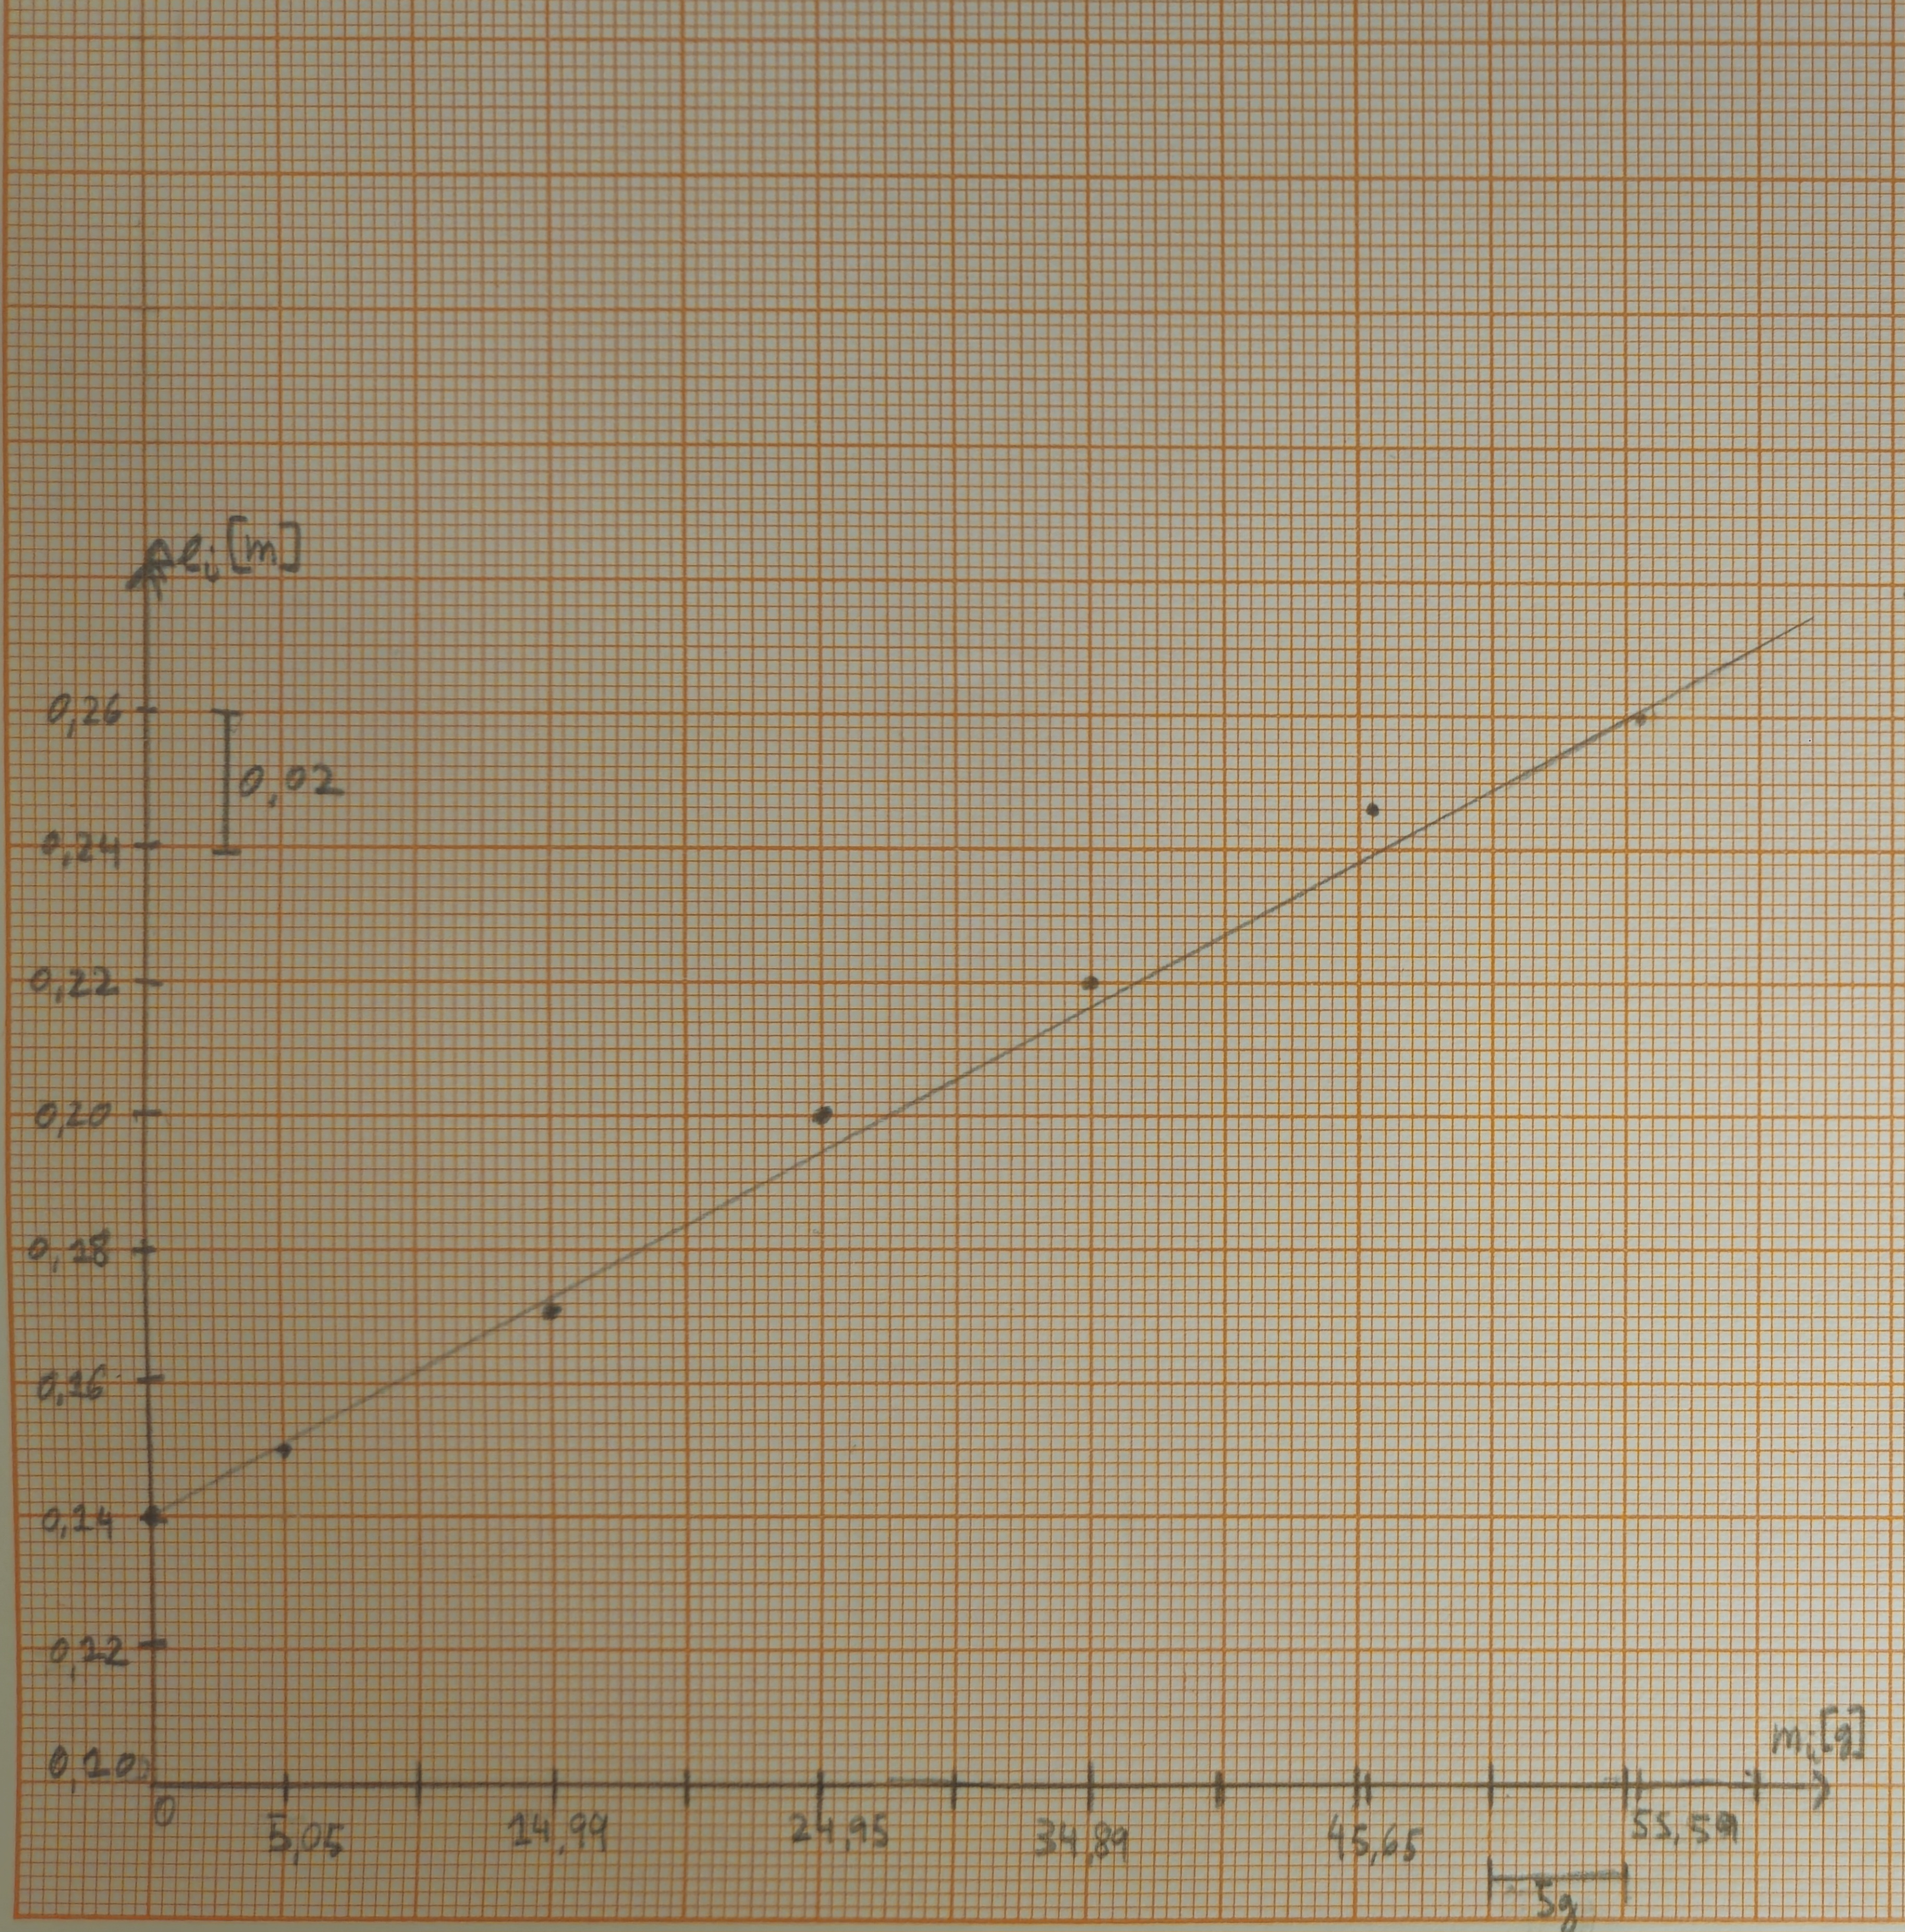
\includegraphics[width=0.65\textwidth, trim={0 0 0 20cm}, clip = true]{fotomolla/Molla 1/m1statico_lm.jpg}
    \caption{Grafico di $\Delta L_i$ vs $M_i$}
\end{figure}

\begin{figure}[!ht]
    \centering
    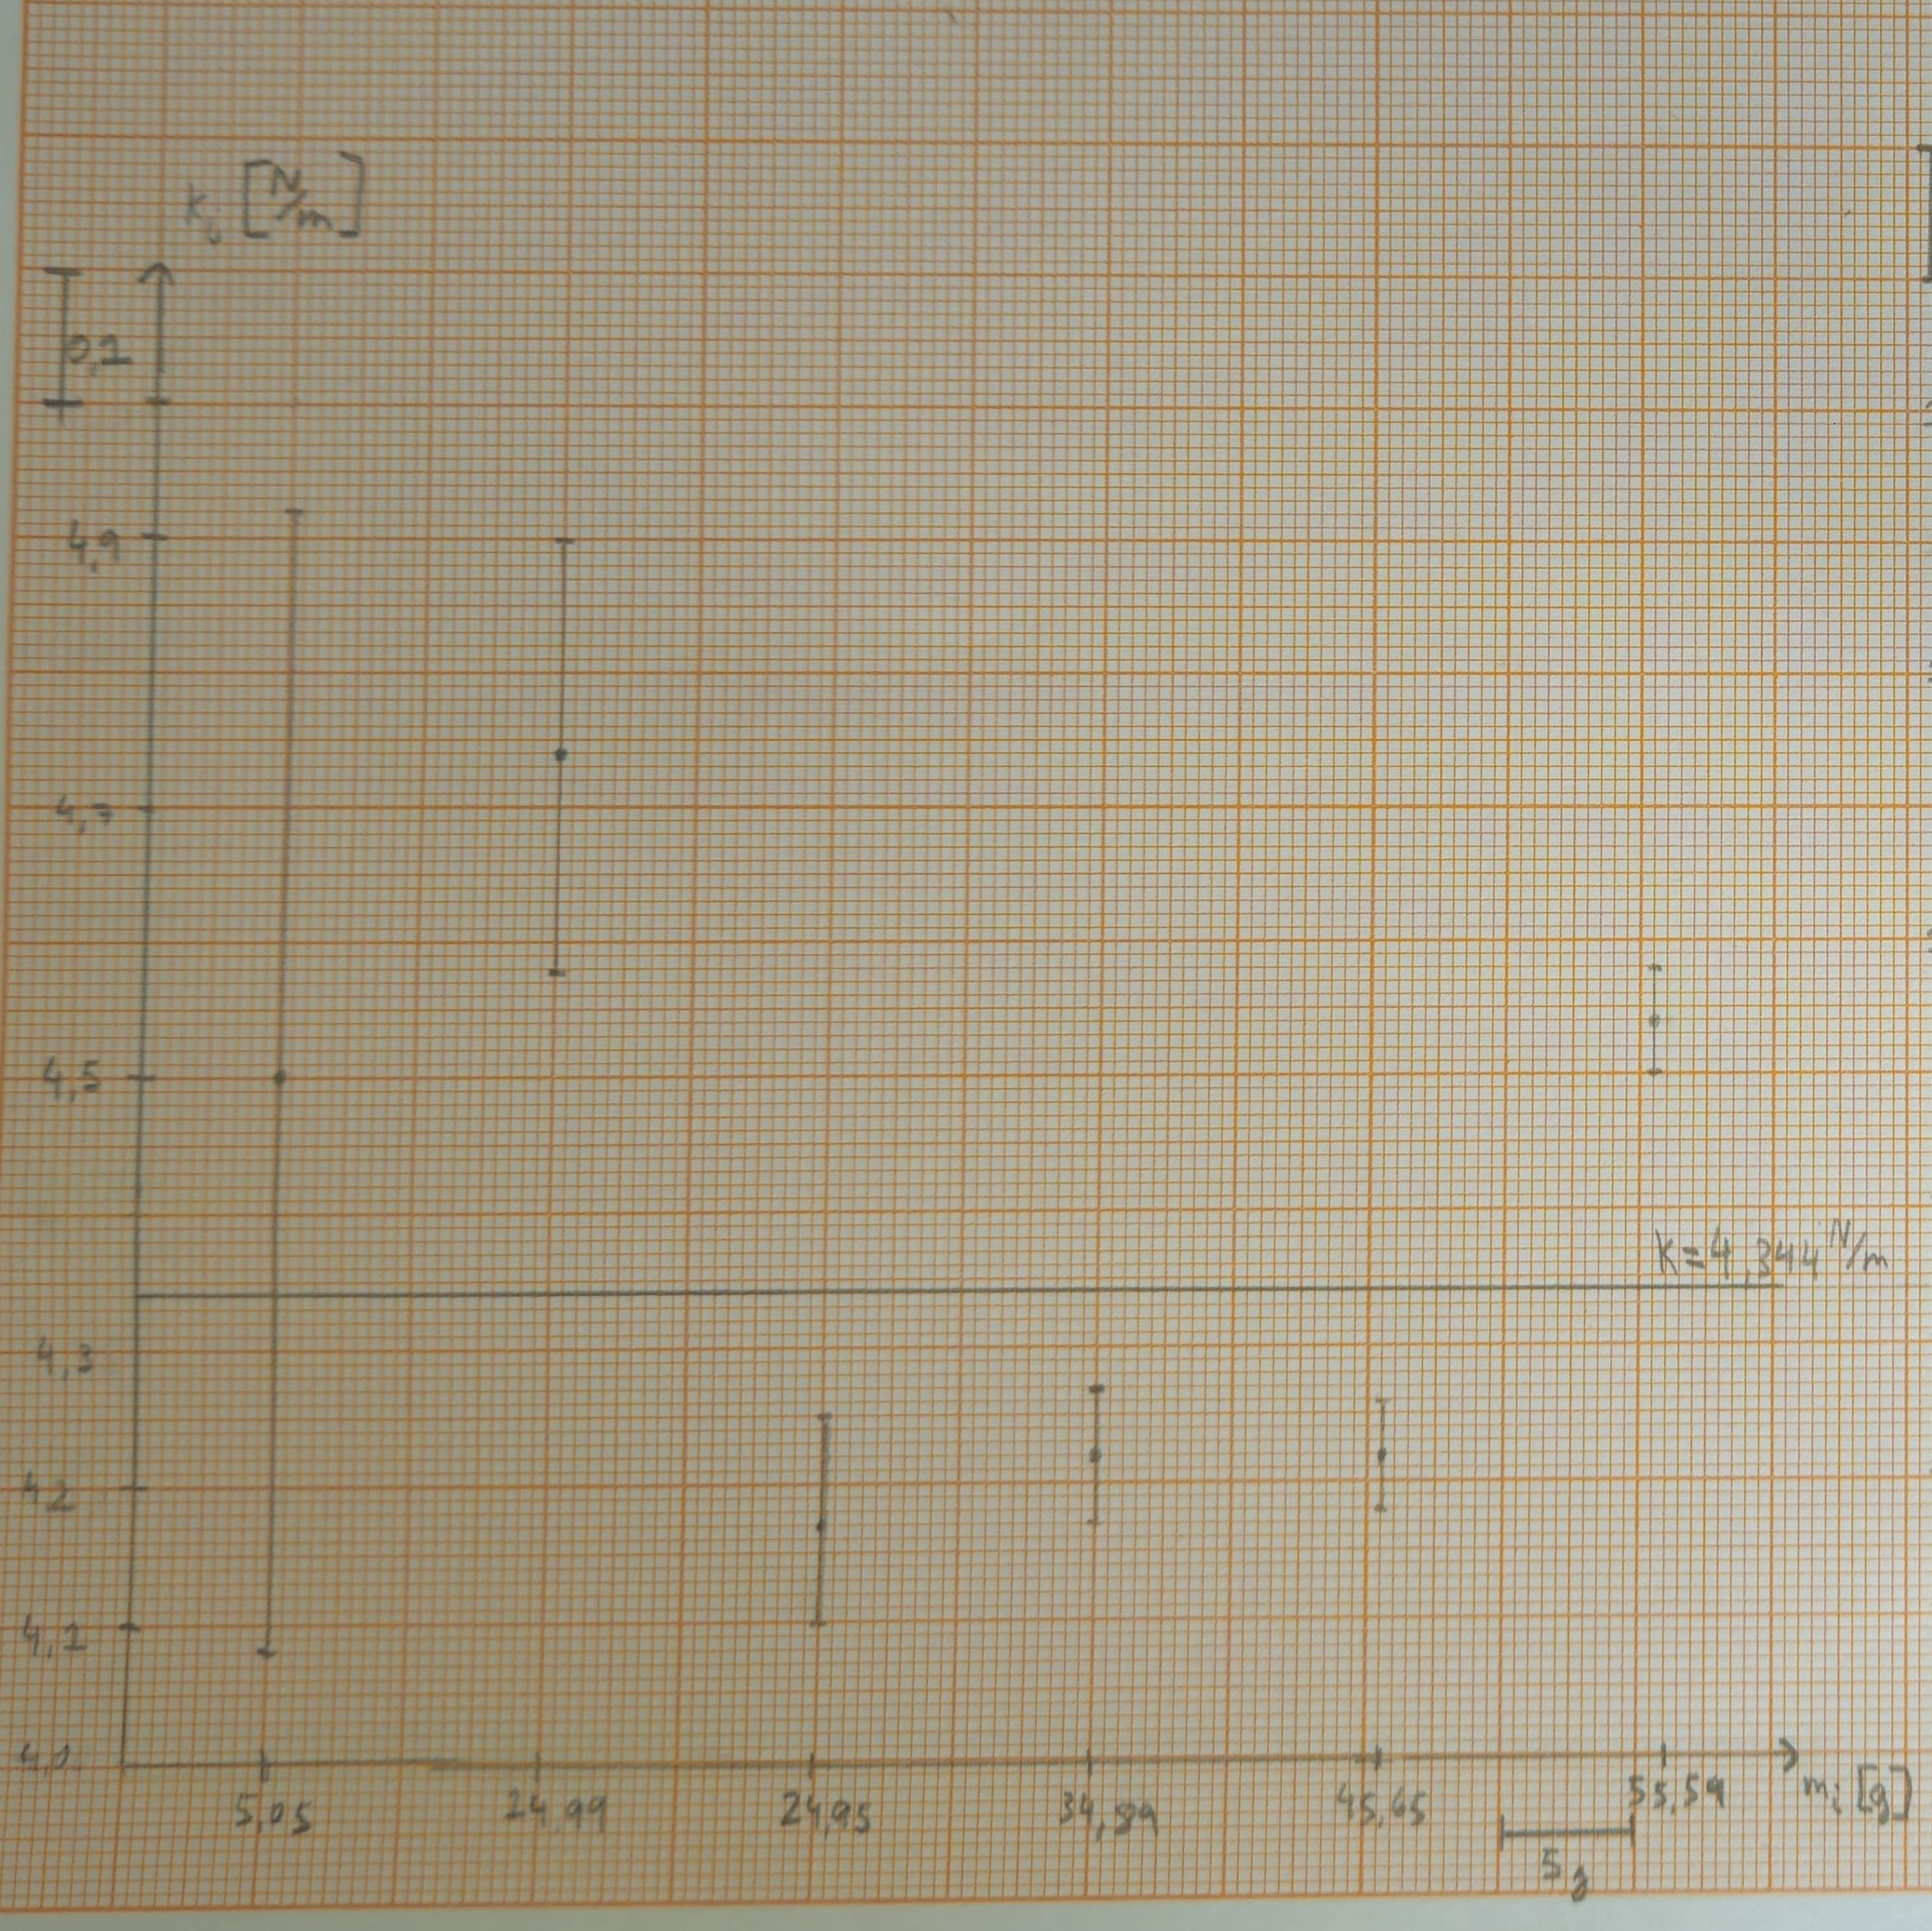
\includegraphics[width=0.65\textwidth]{fotomolla/Molla 1/m1statico_km.jpg}
    \caption{Grafico di $K_i$ vs $M_i$}
\end{figure}

\subsubsection{Metodo Dinamico}
\begin{figure}[!ht]
    \centering
    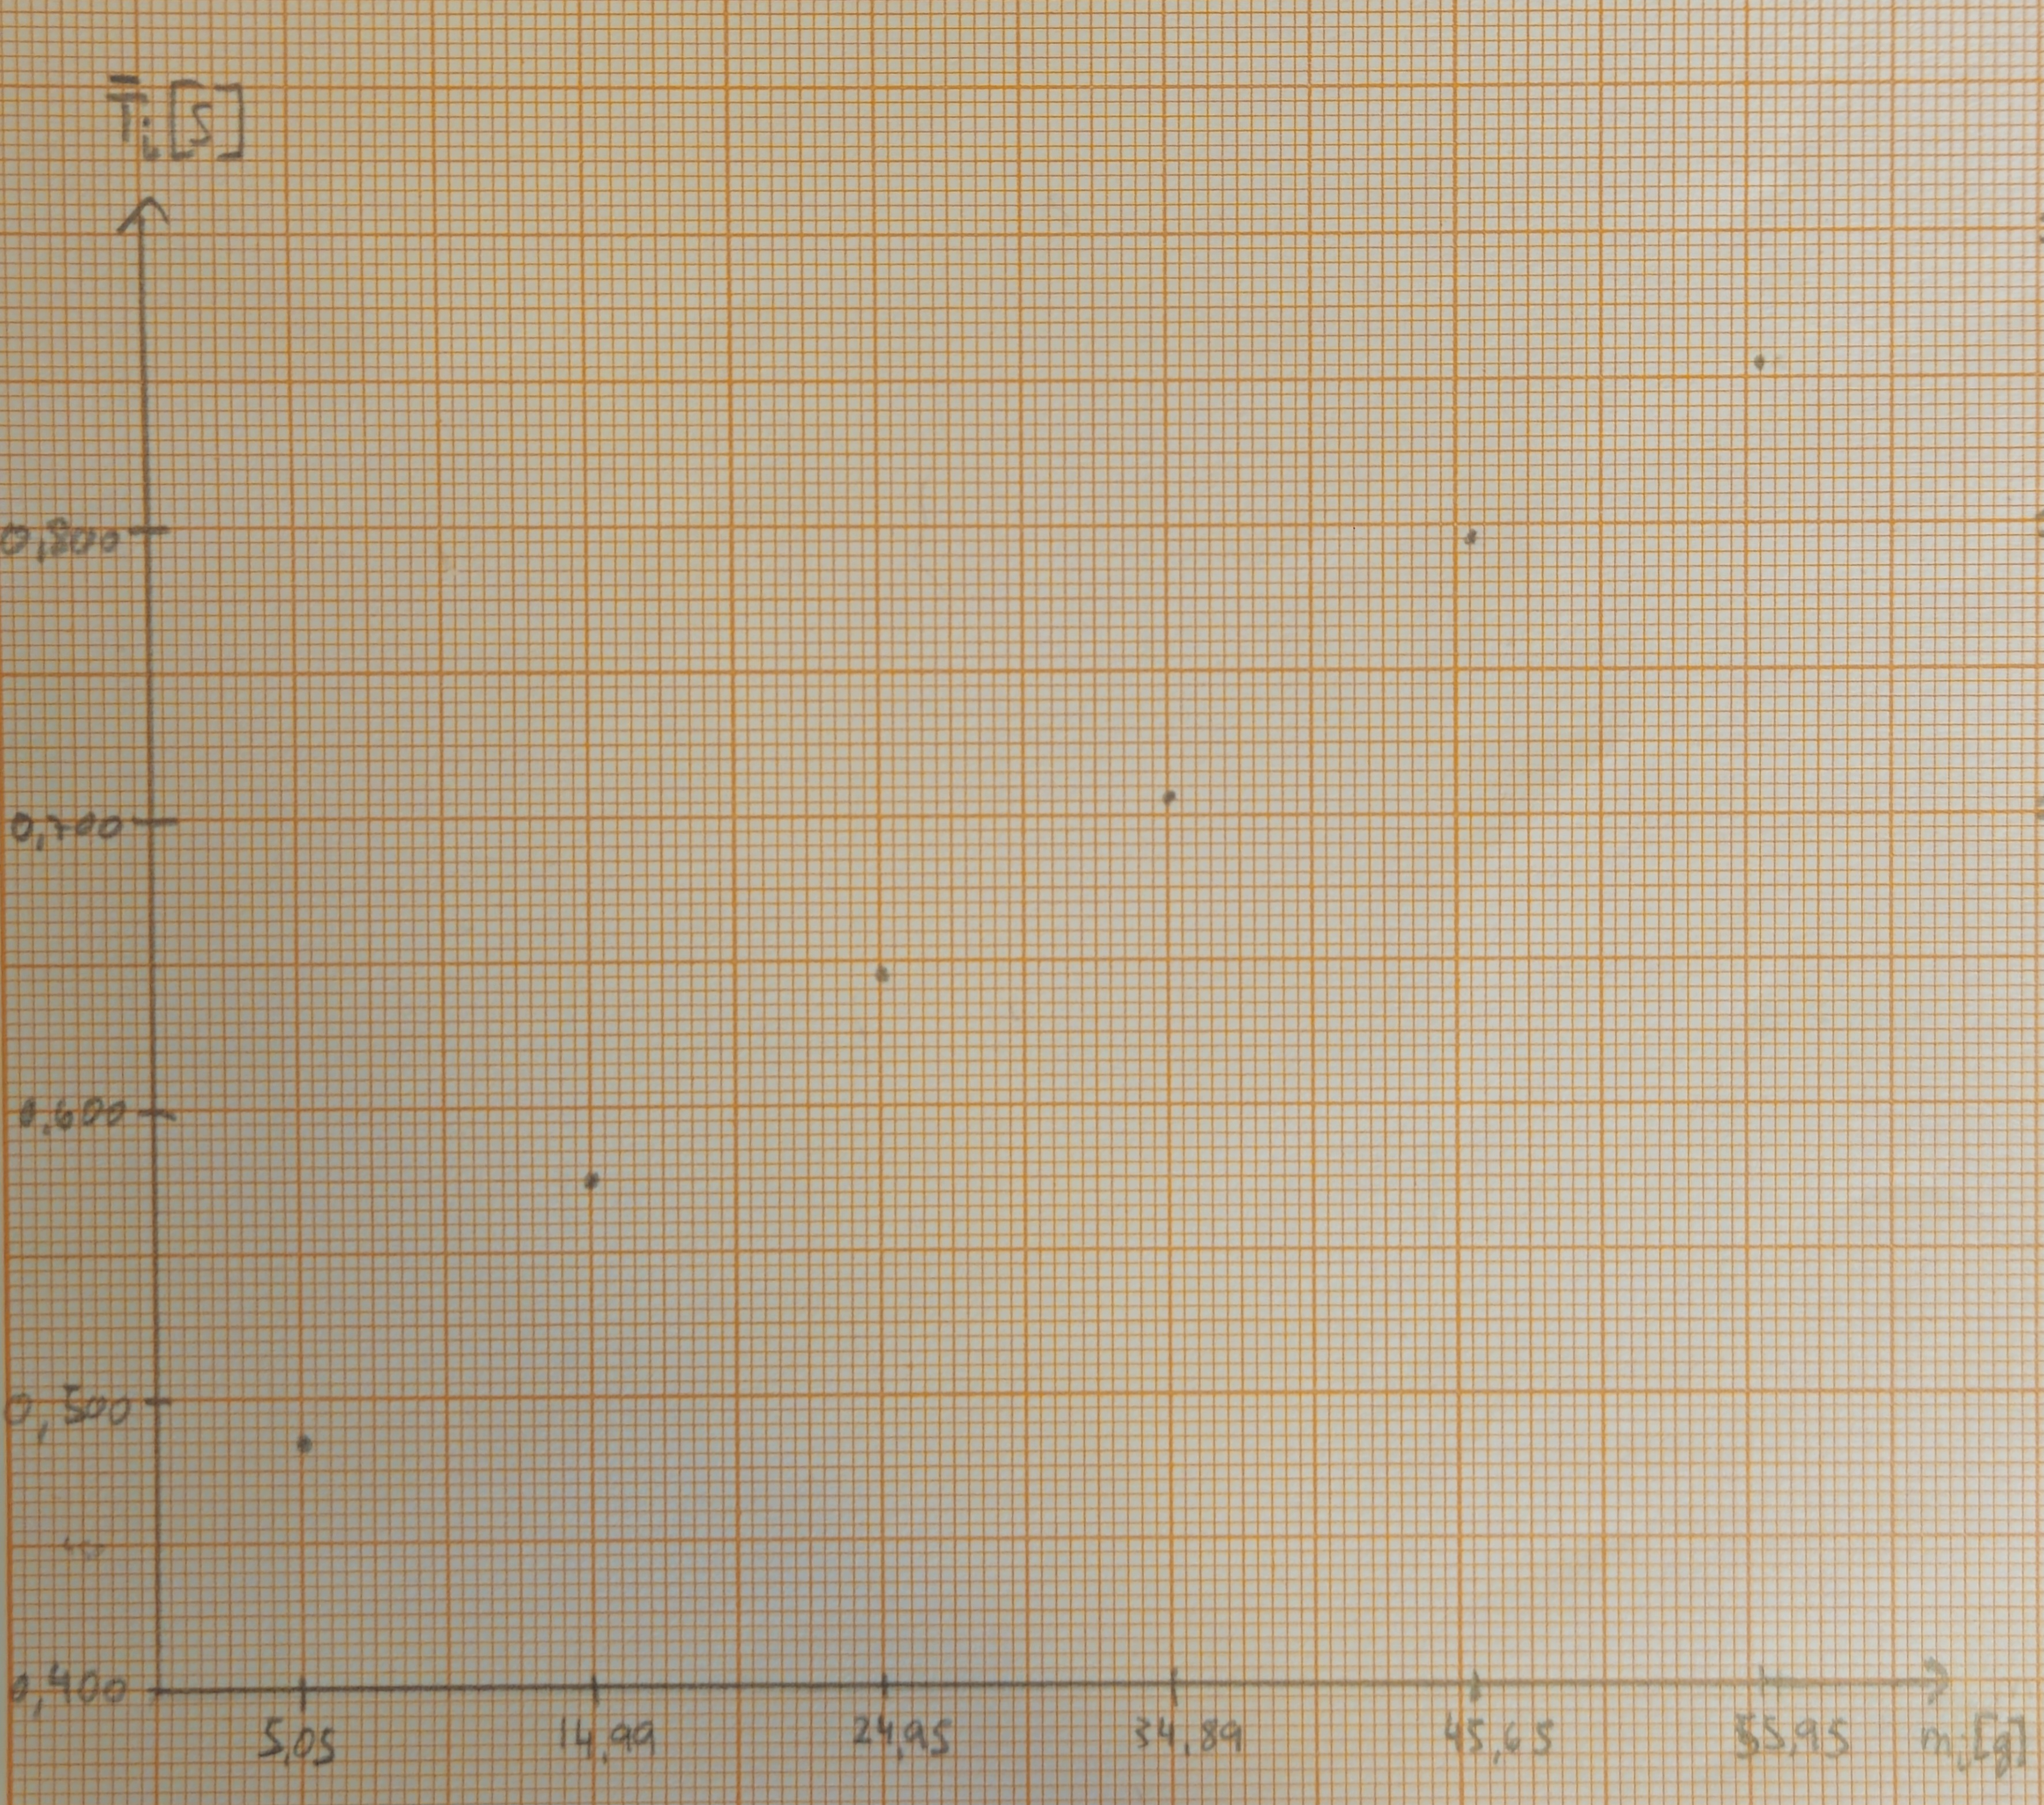
\includegraphics[width=0.65\textwidth]{fotomolla/Molla 1/m1dinamico_tm.jpg}
    \caption{Grafico di $\bar{T}_i$ vs $M_i$}
\end{figure}

\begin{figure}[!ht]
    \centering
    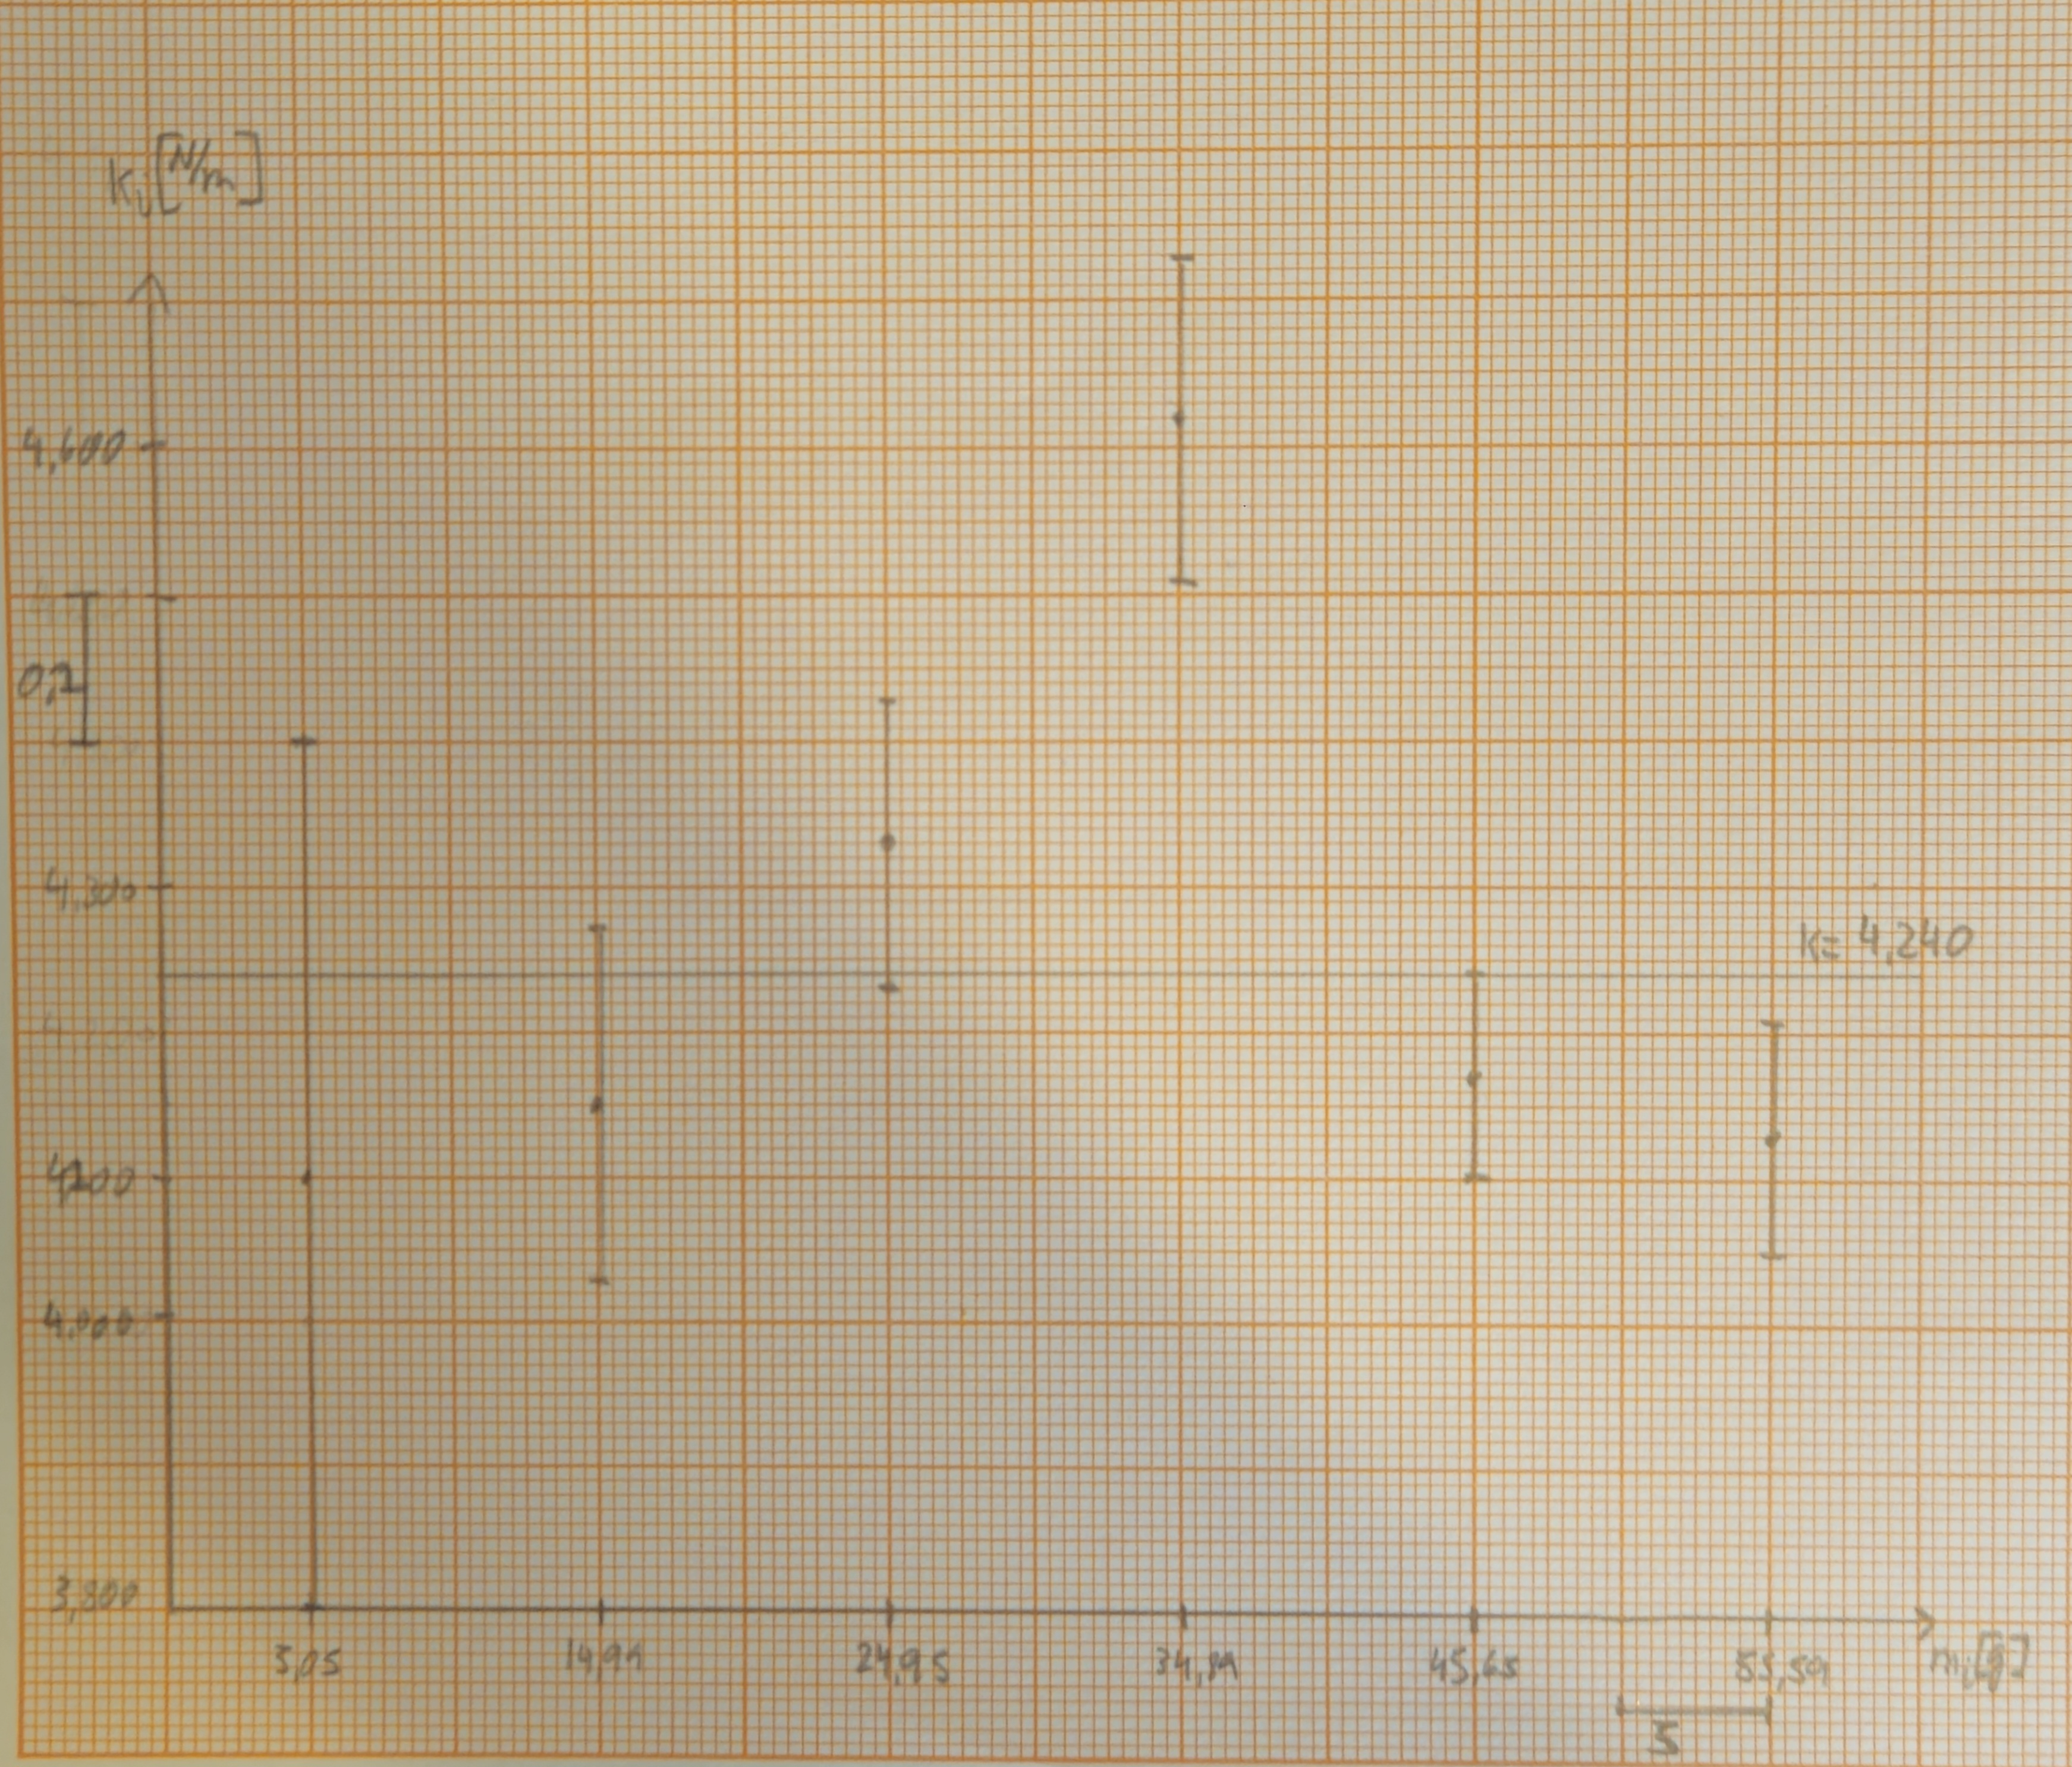
\includegraphics[width=0.65\textwidth]{fotomolla/Molla 1/m1dinamico_diffperiodo.jpg}
    \caption{Grafico di $k_1$ con modello differenza periodi}
\end{figure}

\begin{figure}[!ht]
    \centering
    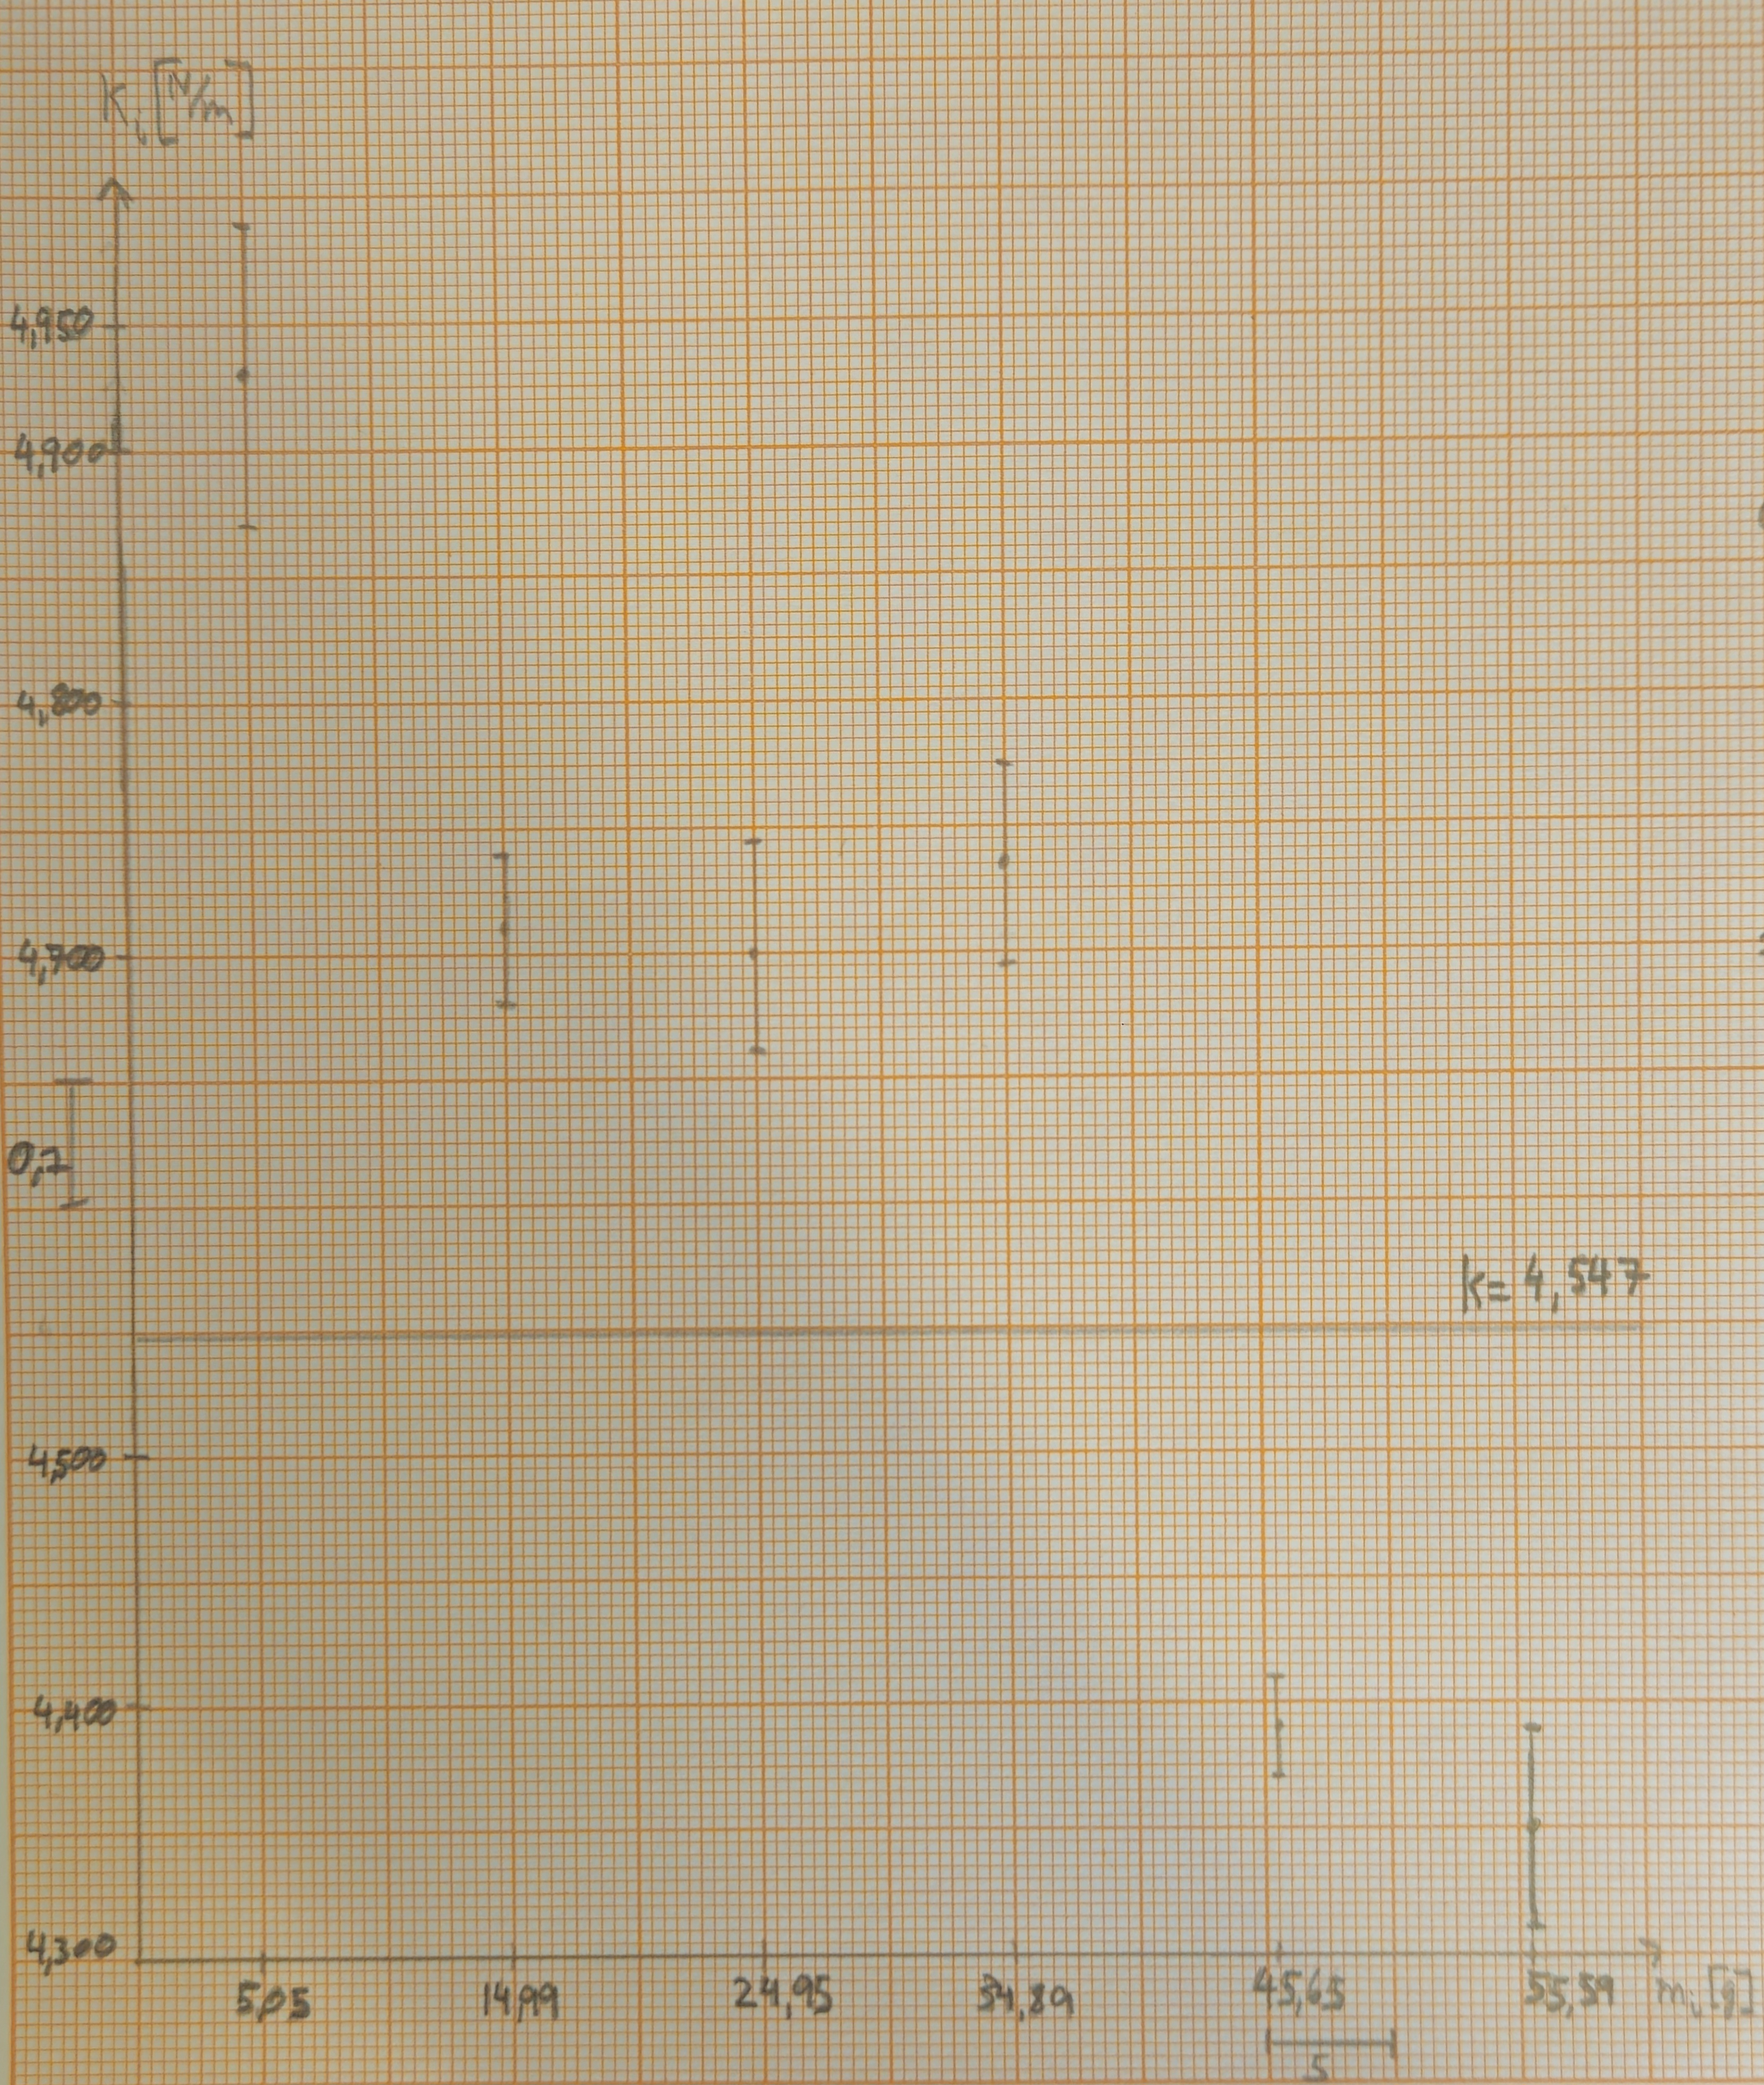
\includegraphics[width=0.65\textwidth]{fotomolla/Molla 1/m1dinamico_mefficace.jpg}
    \caption{Grafico di $k_1$ con modello $m_{eff}$}
\end{figure}
\FloatBarrier

\subsubsection{Istogrammi}
\FloatBarrier
\begin{figure}[!htbp]
    \begin{minipage}[b]{0.45\textwidth}
        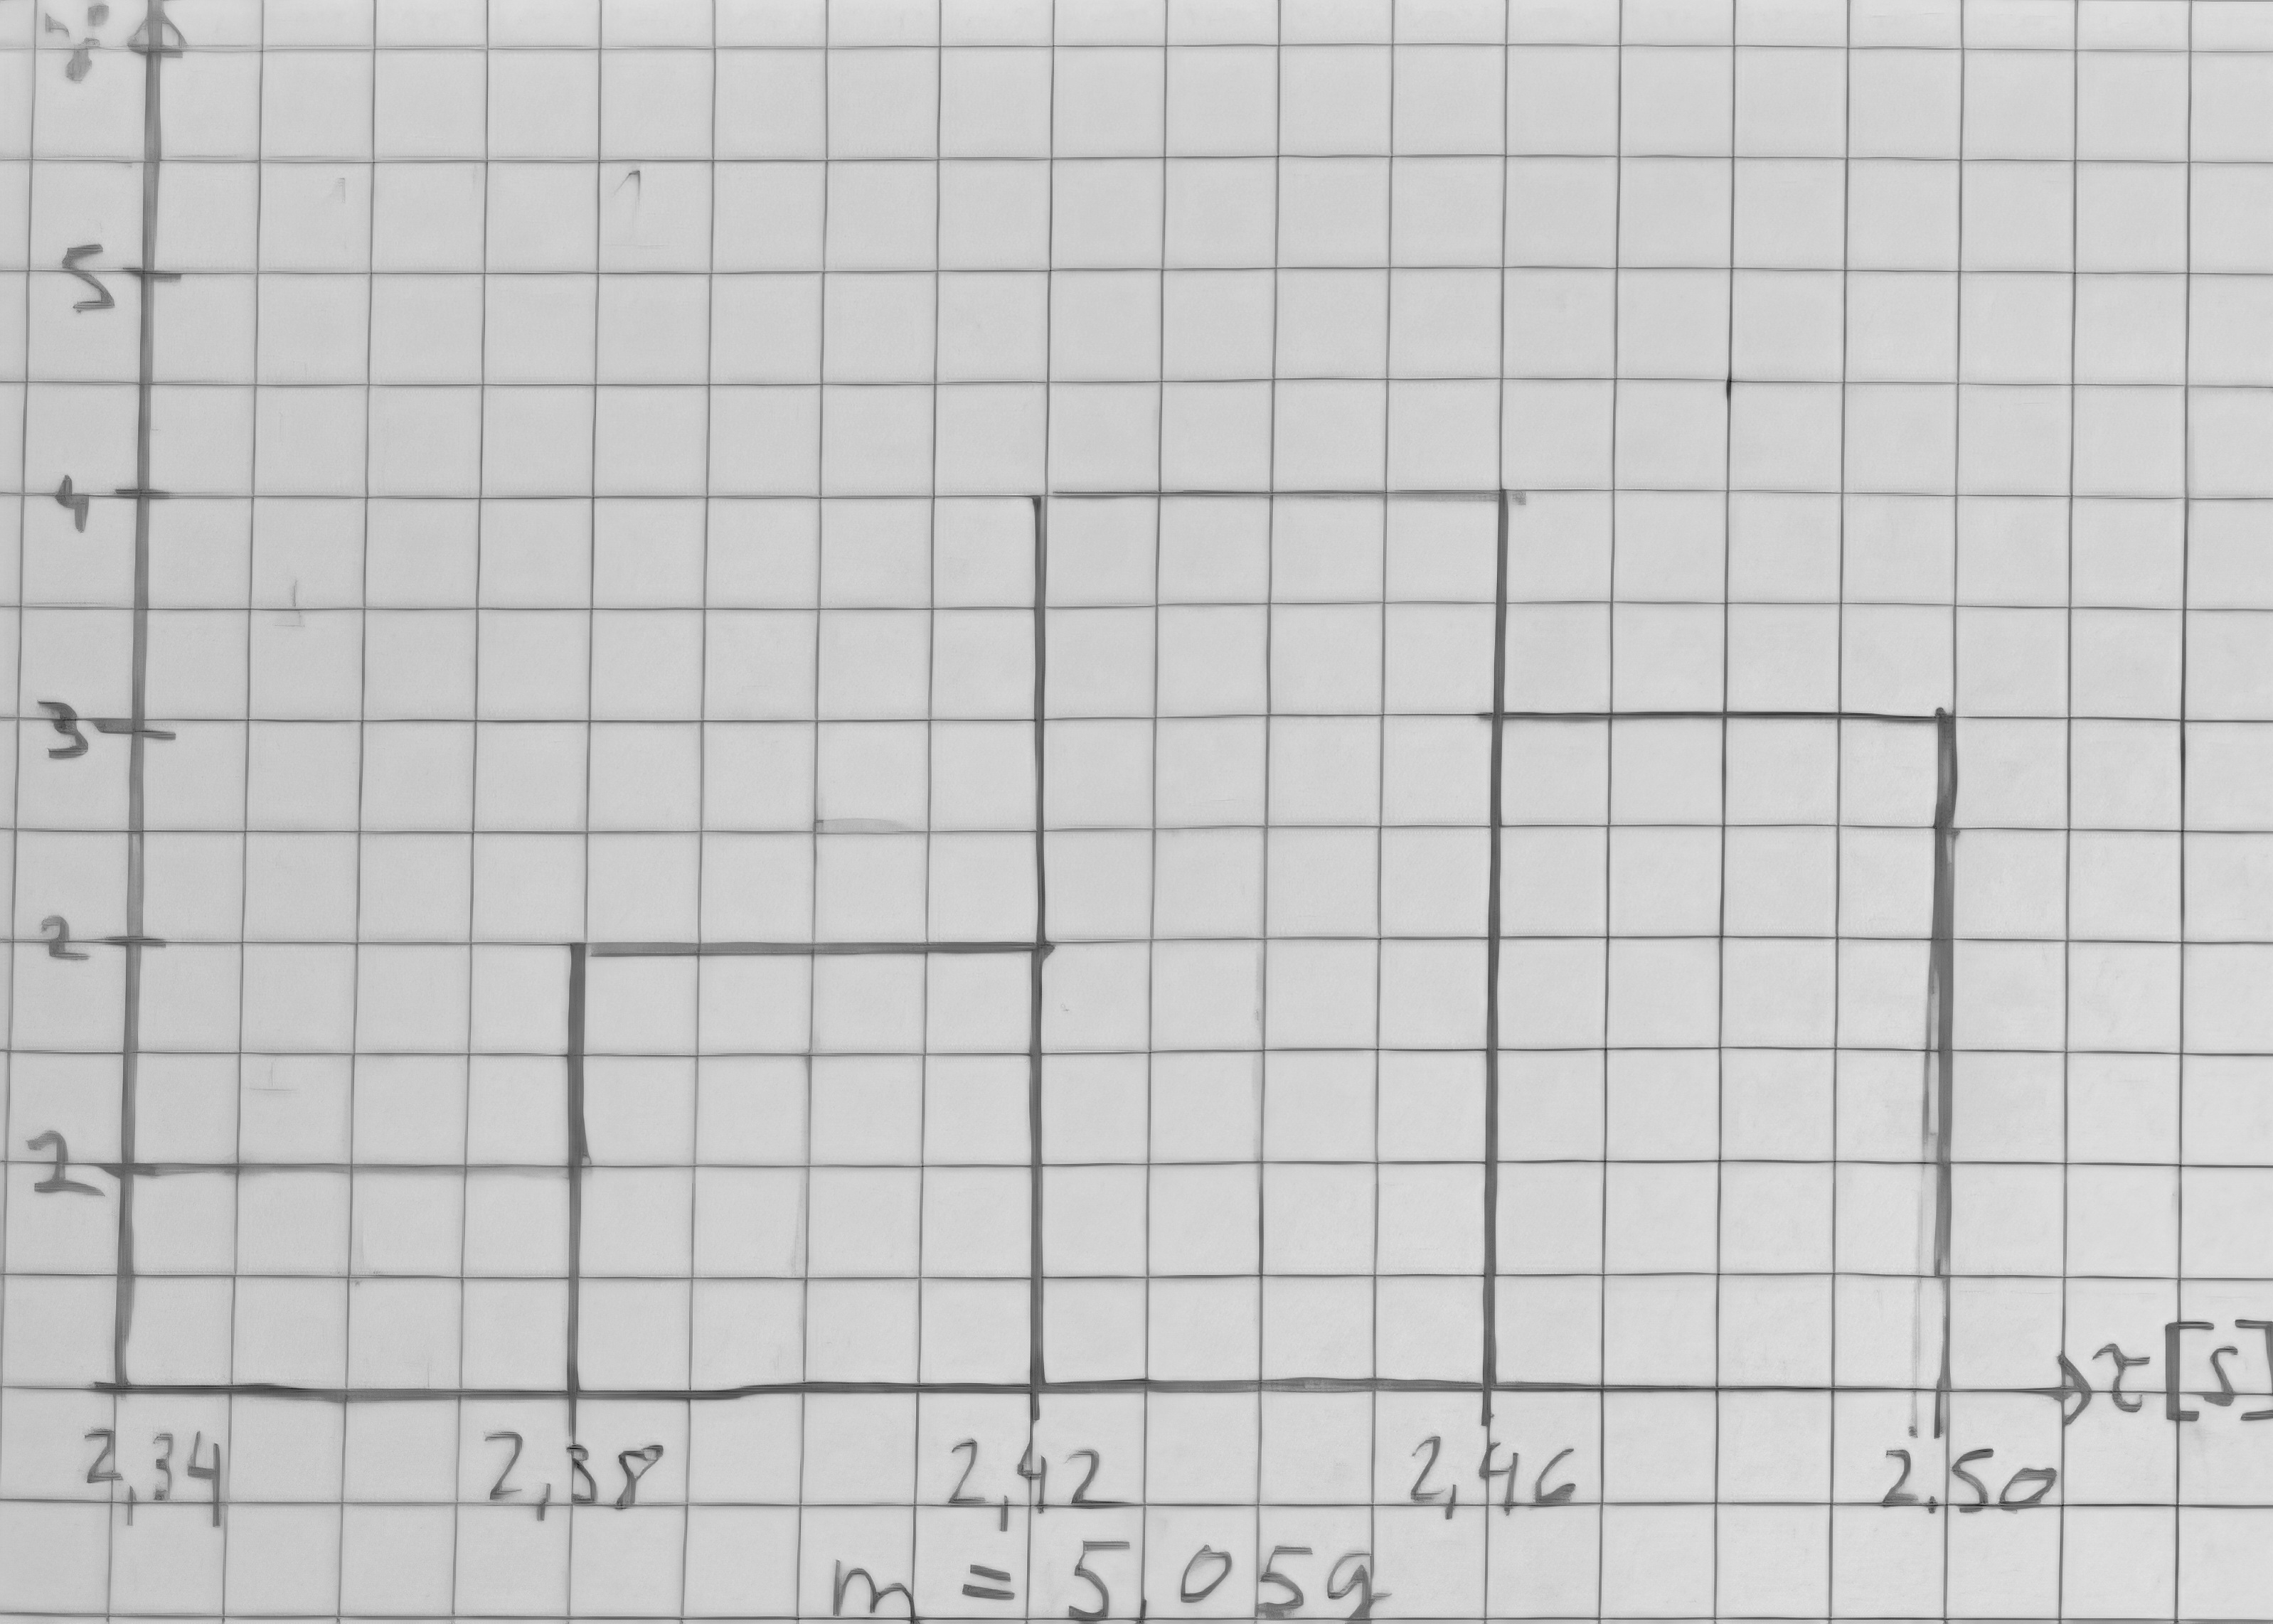
\includegraphics[width=\textwidth]{fotomolla/Molla 1/5.05.jpg}
        \caption{Misure con $m=\SI{5.05}{g}$}
    \end{minipage}
    \hfil
     \begin{minipage}[b]{0.45\textwidth}
        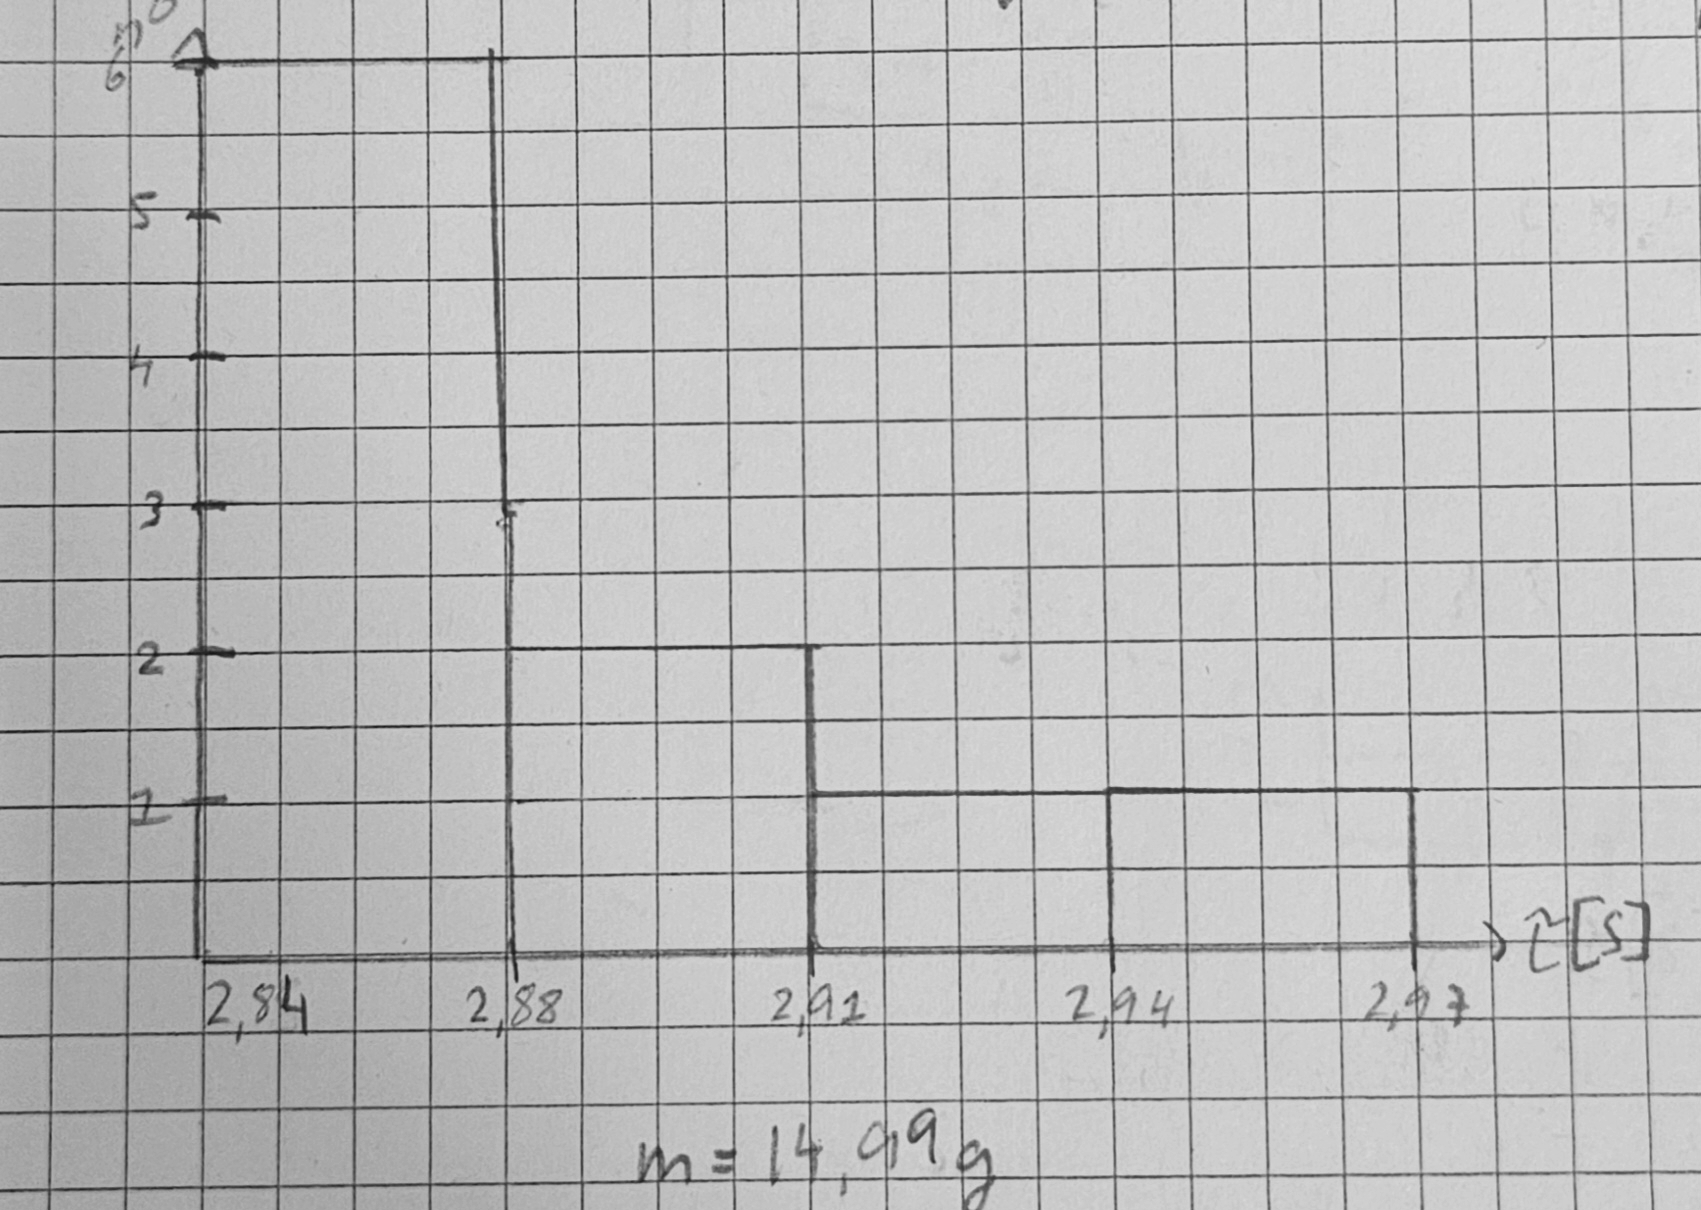
\includegraphics[width=\textwidth]{fotomolla/Molla 1/14.99.jpg}
        \caption{Misure con $m=\SI{14.99}{g}$}
    \end{minipage}
\end{figure}

\begin{figure}[!htbp]
    \begin{minipage}[b]{0.45\textwidth}
        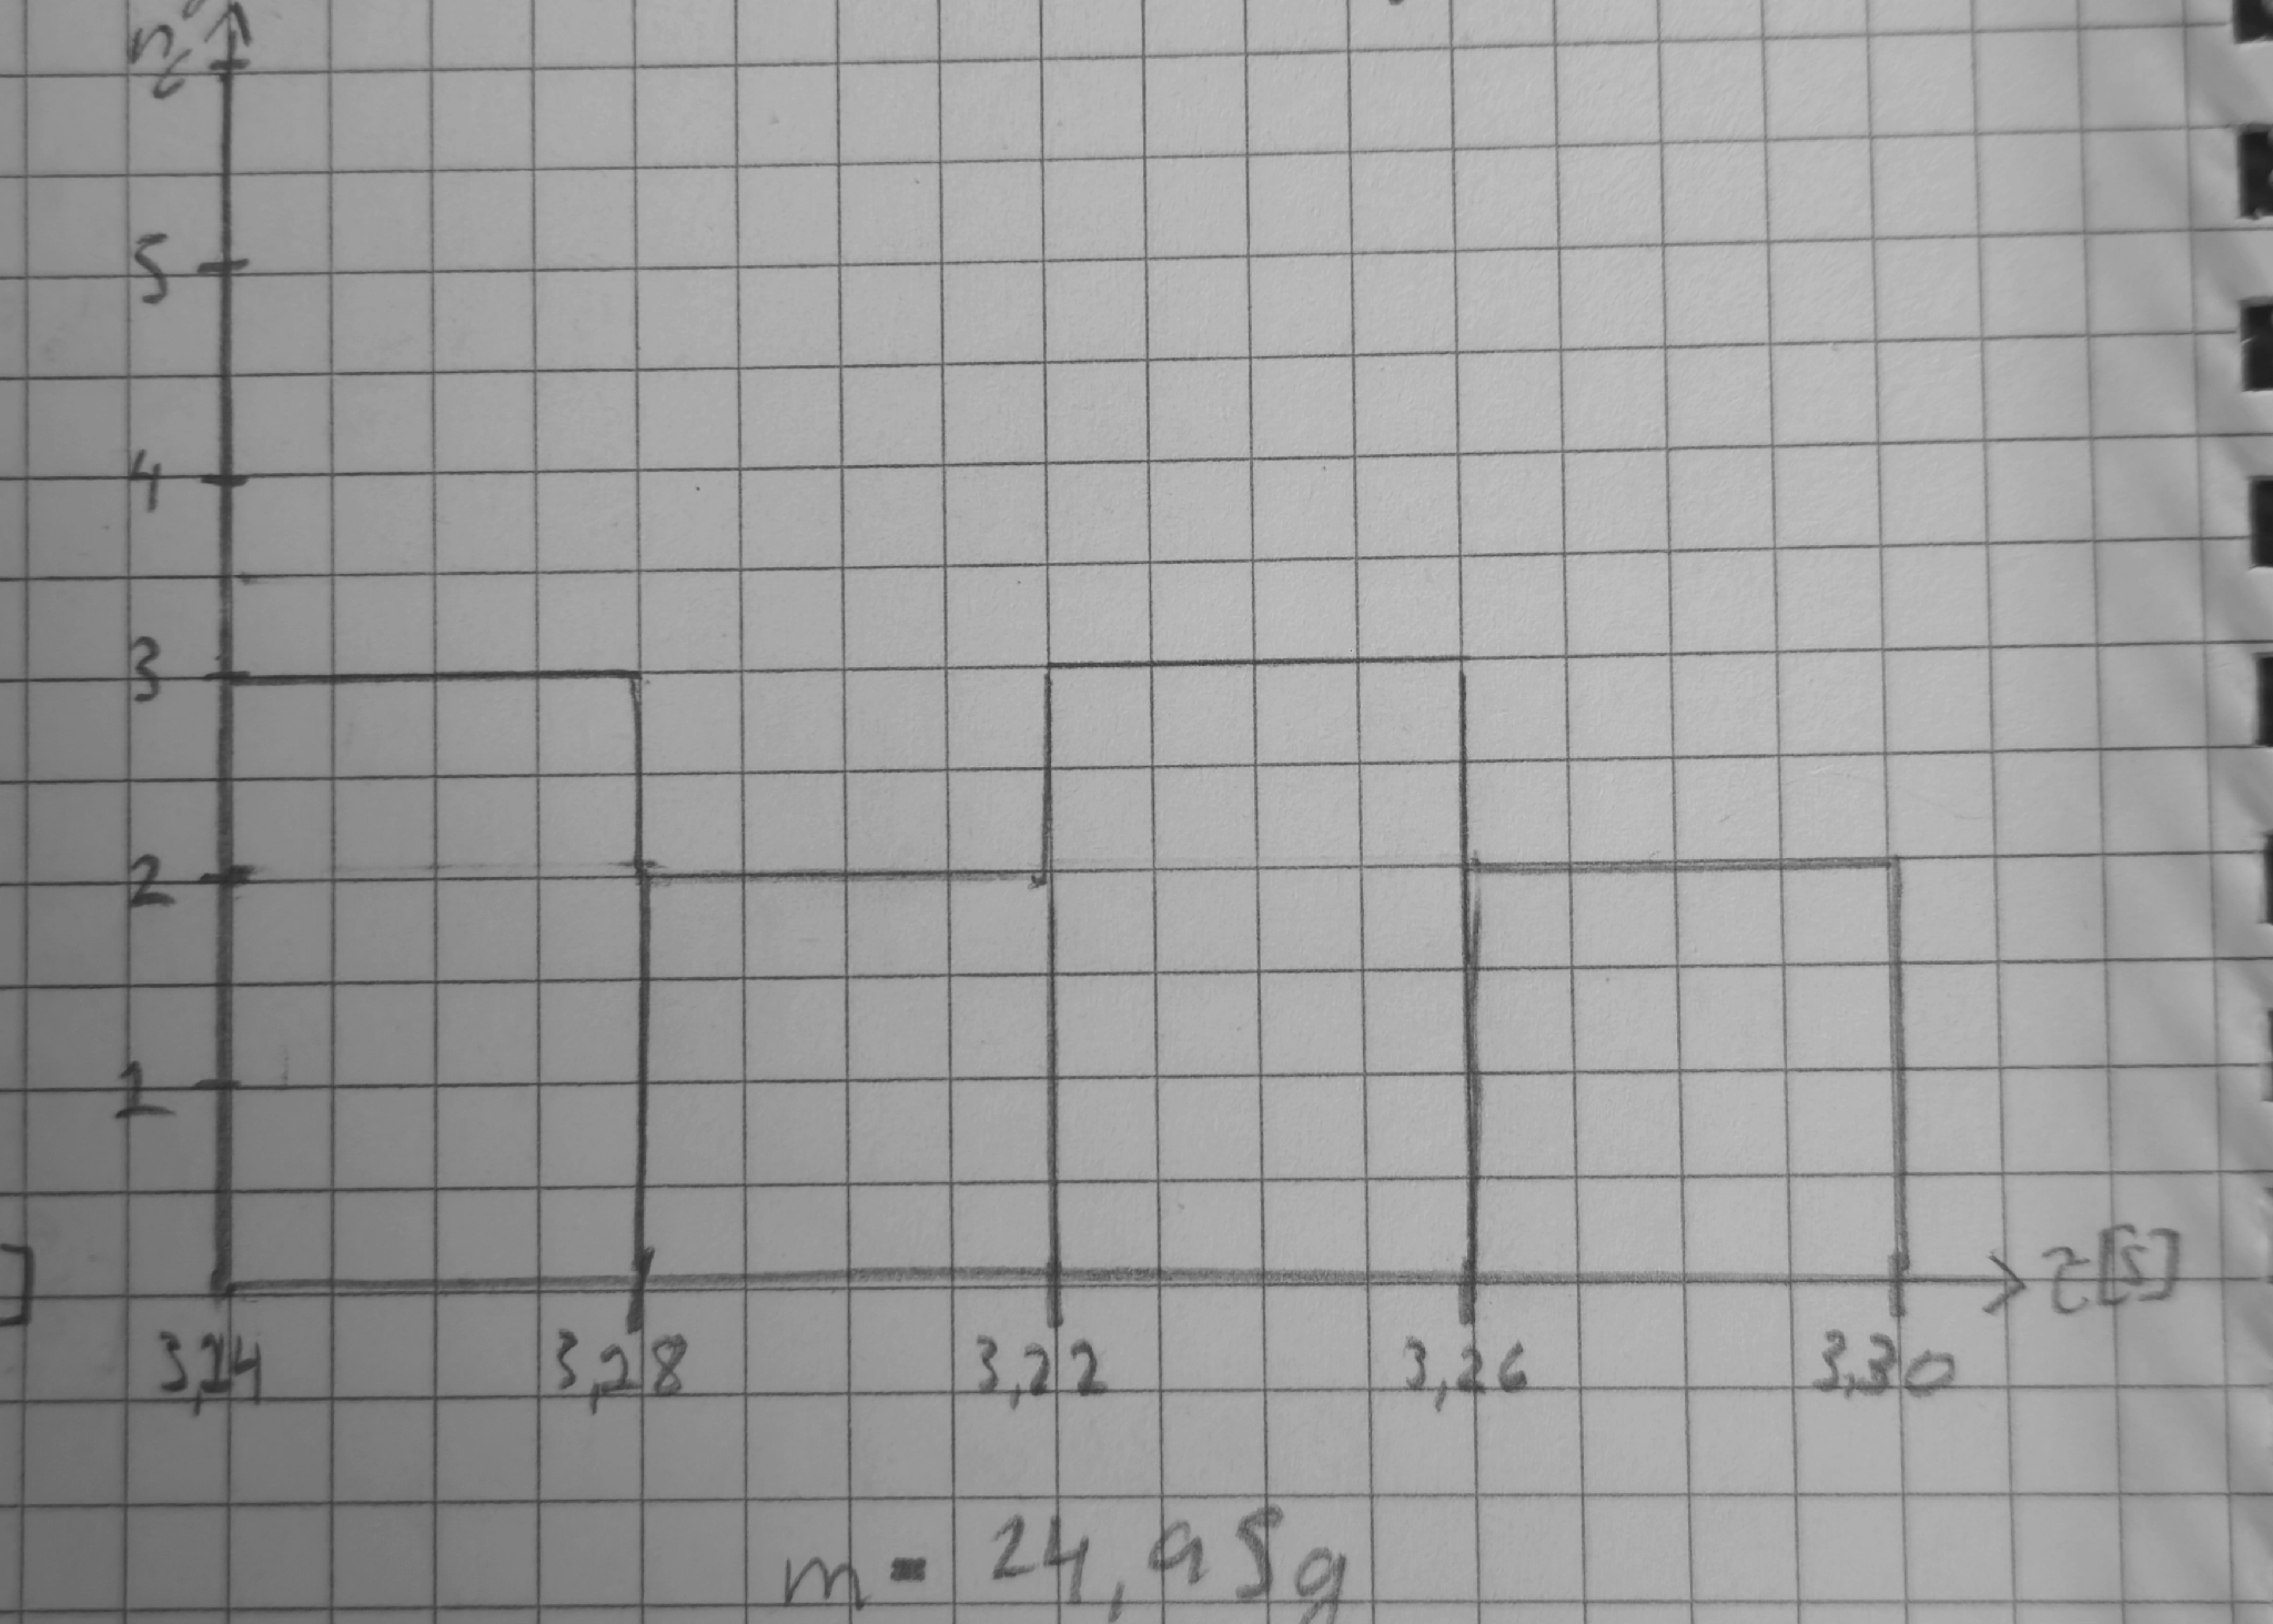
\includegraphics[width=\textwidth]{fotomolla/Molla 1/25.jpg}
        \caption{Misure con $m=\SI{24.95}{g}$}
    \end{minipage}
    \hfil
     \begin{minipage}[b]{0.45\textwidth}
        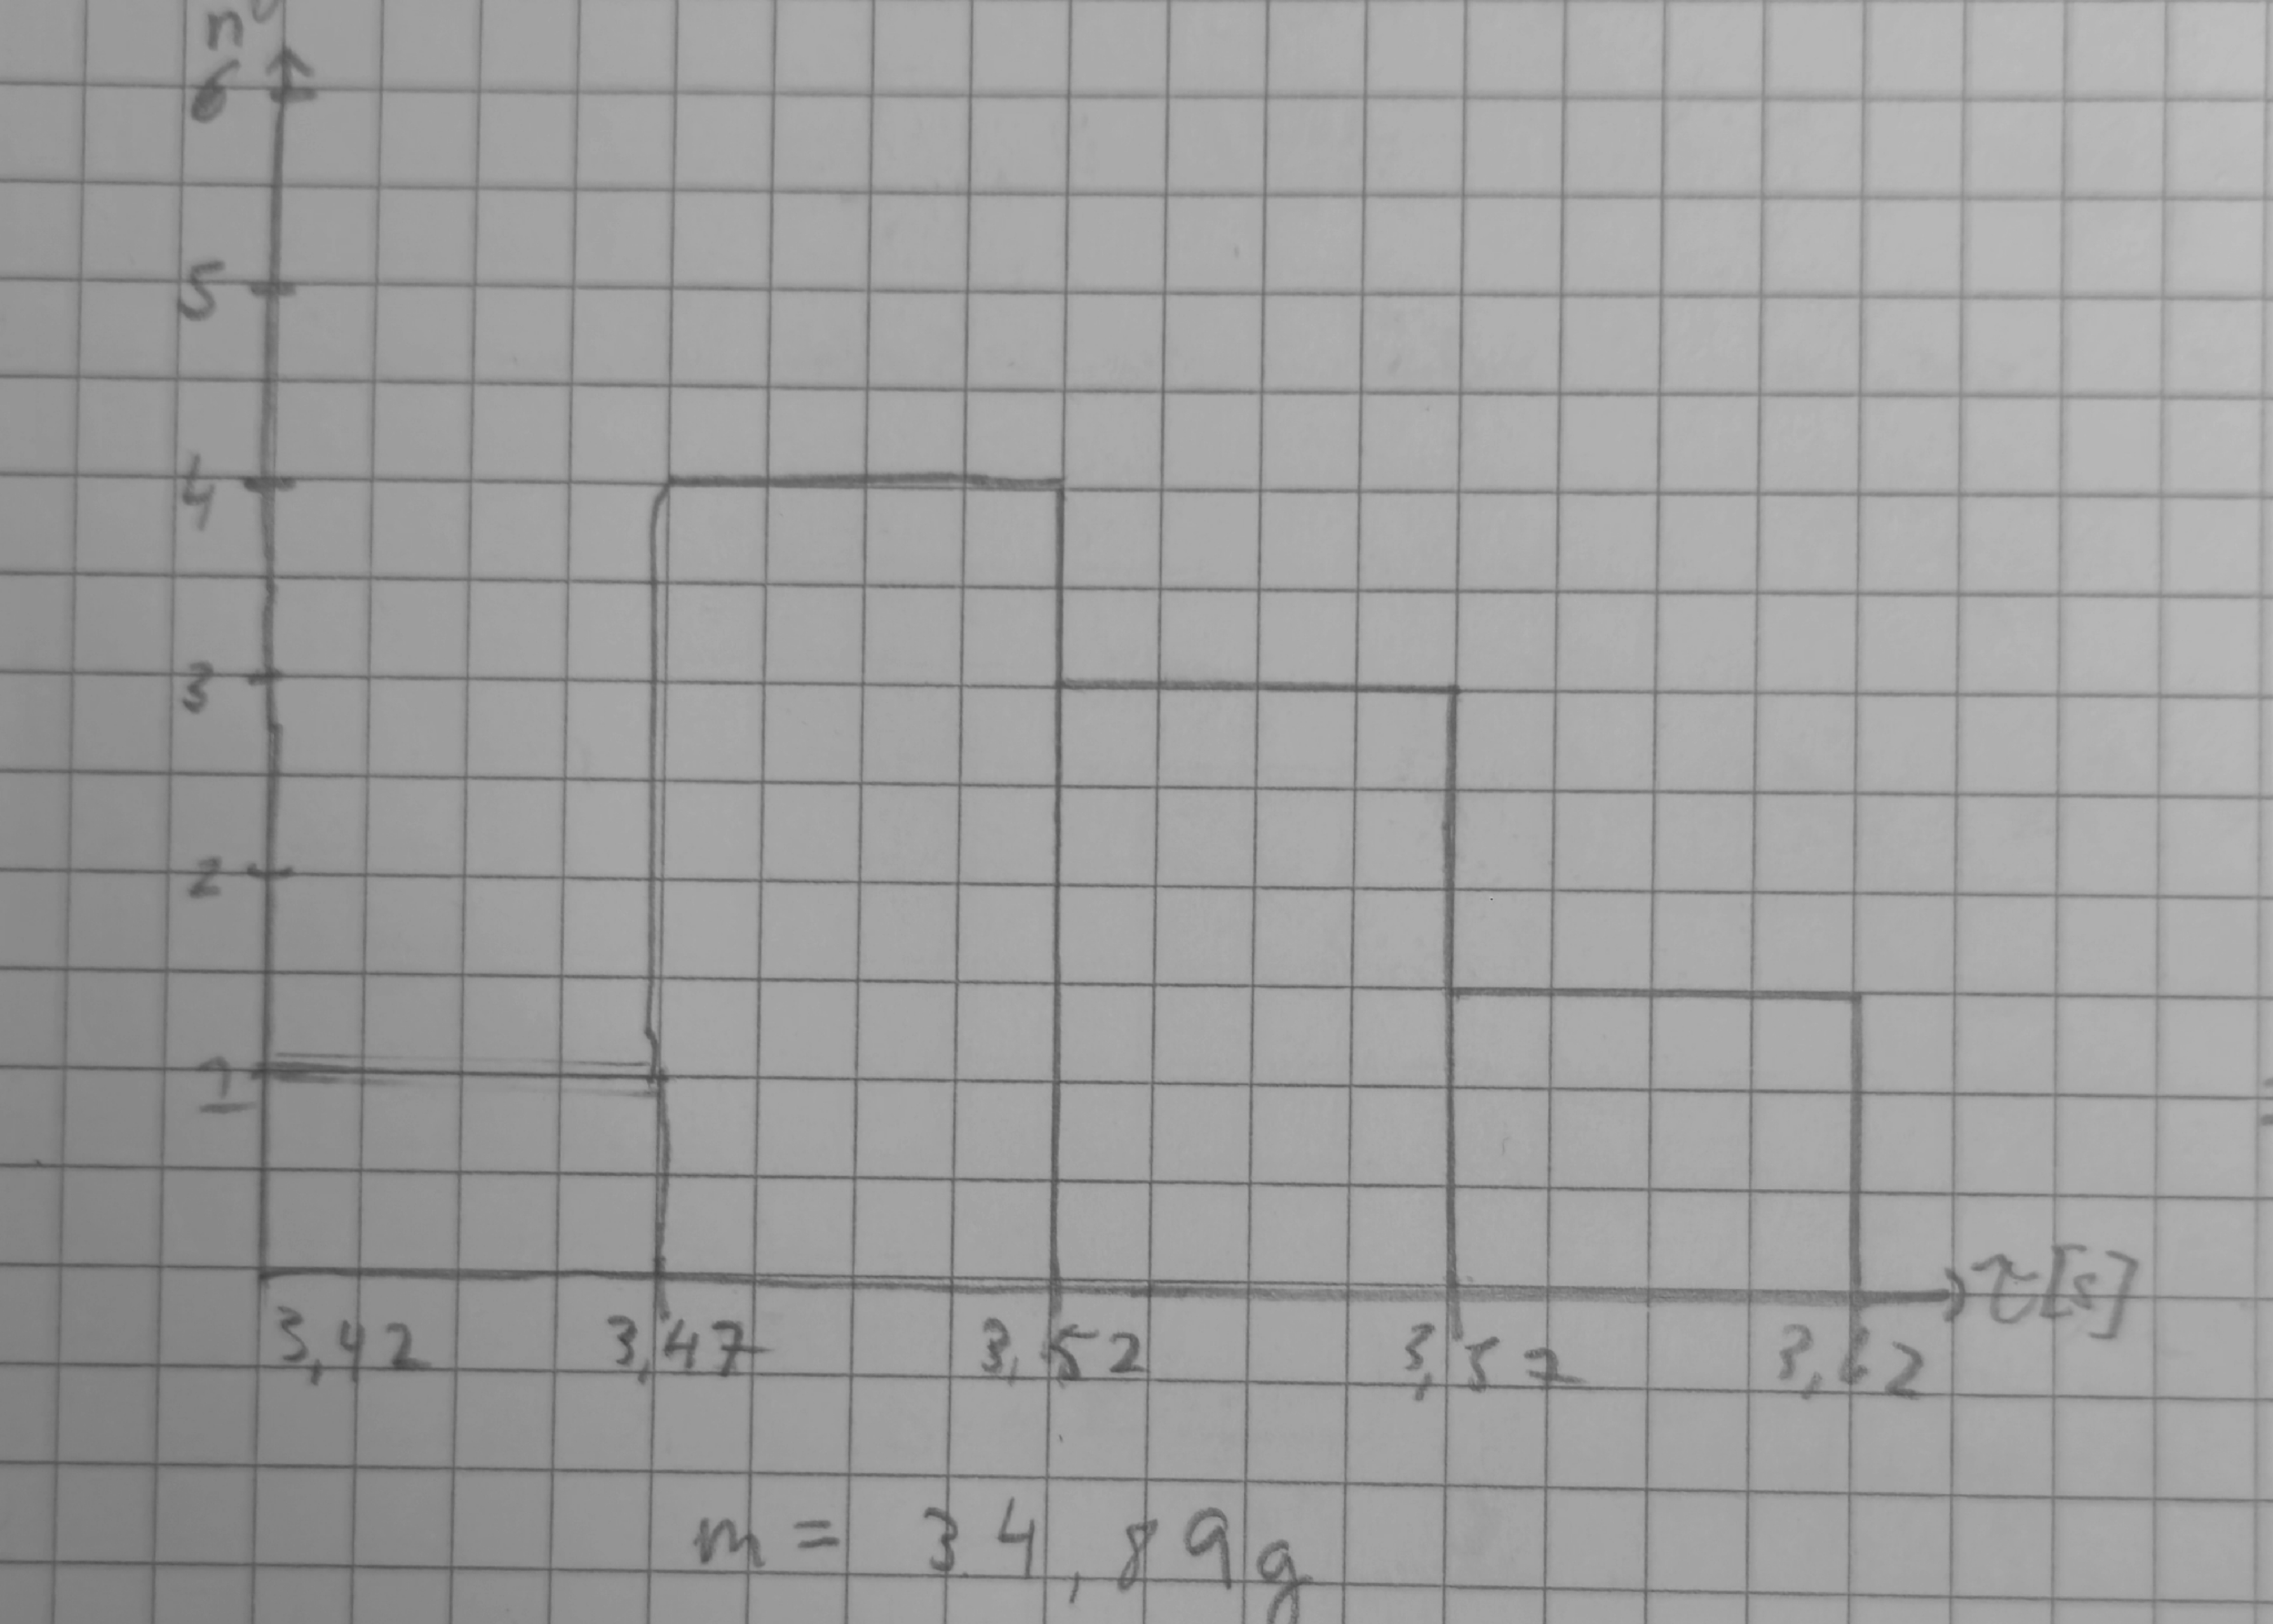
\includegraphics[width=\textwidth]{fotomolla/Molla 1/35.jpg}
        \caption{Misure con $m=\SI{34.89}{g}$}
    \end{minipage}
\end{figure}
\begin{figure}[!htbp]
    \begin{minipage}[b]{0.45\textwidth}
        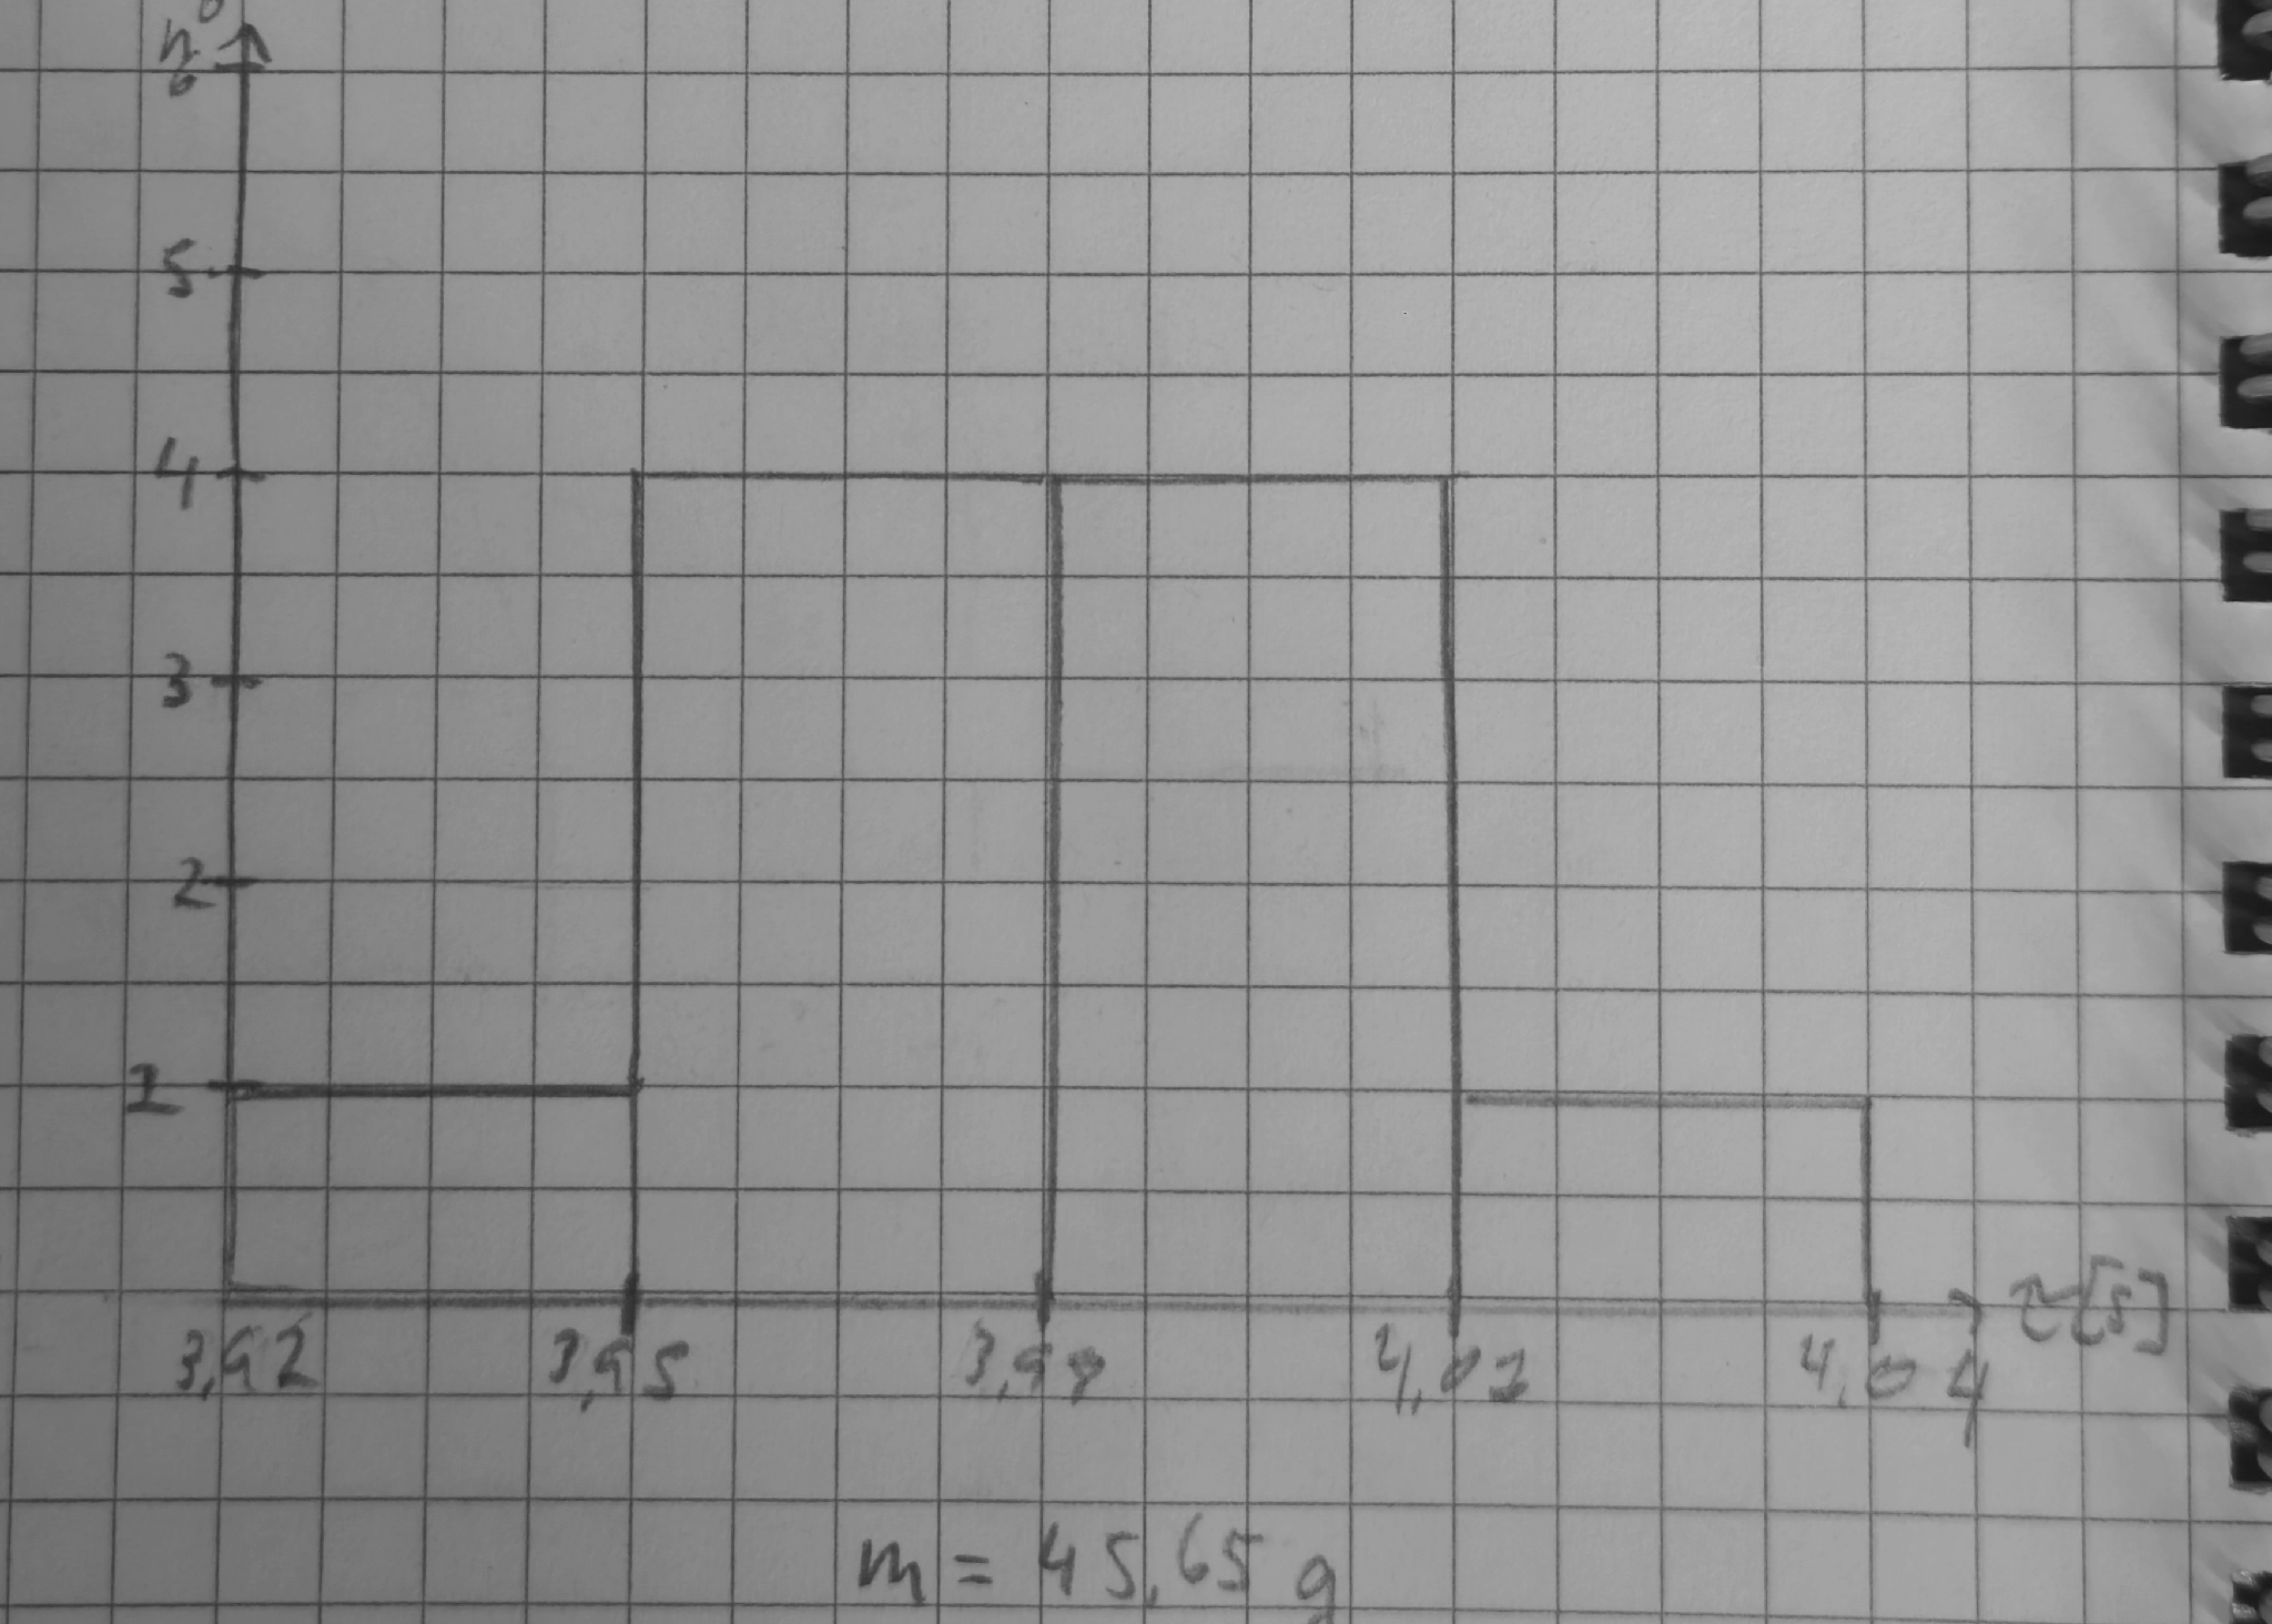
\includegraphics[width=\textwidth]{fotomolla/Molla 1/45.jpg}
        \caption{Misure con $m=\SI{45.65}{g}$}
    \end{minipage}
    \hfil
     \begin{minipage}[b]{0.45\textwidth}
        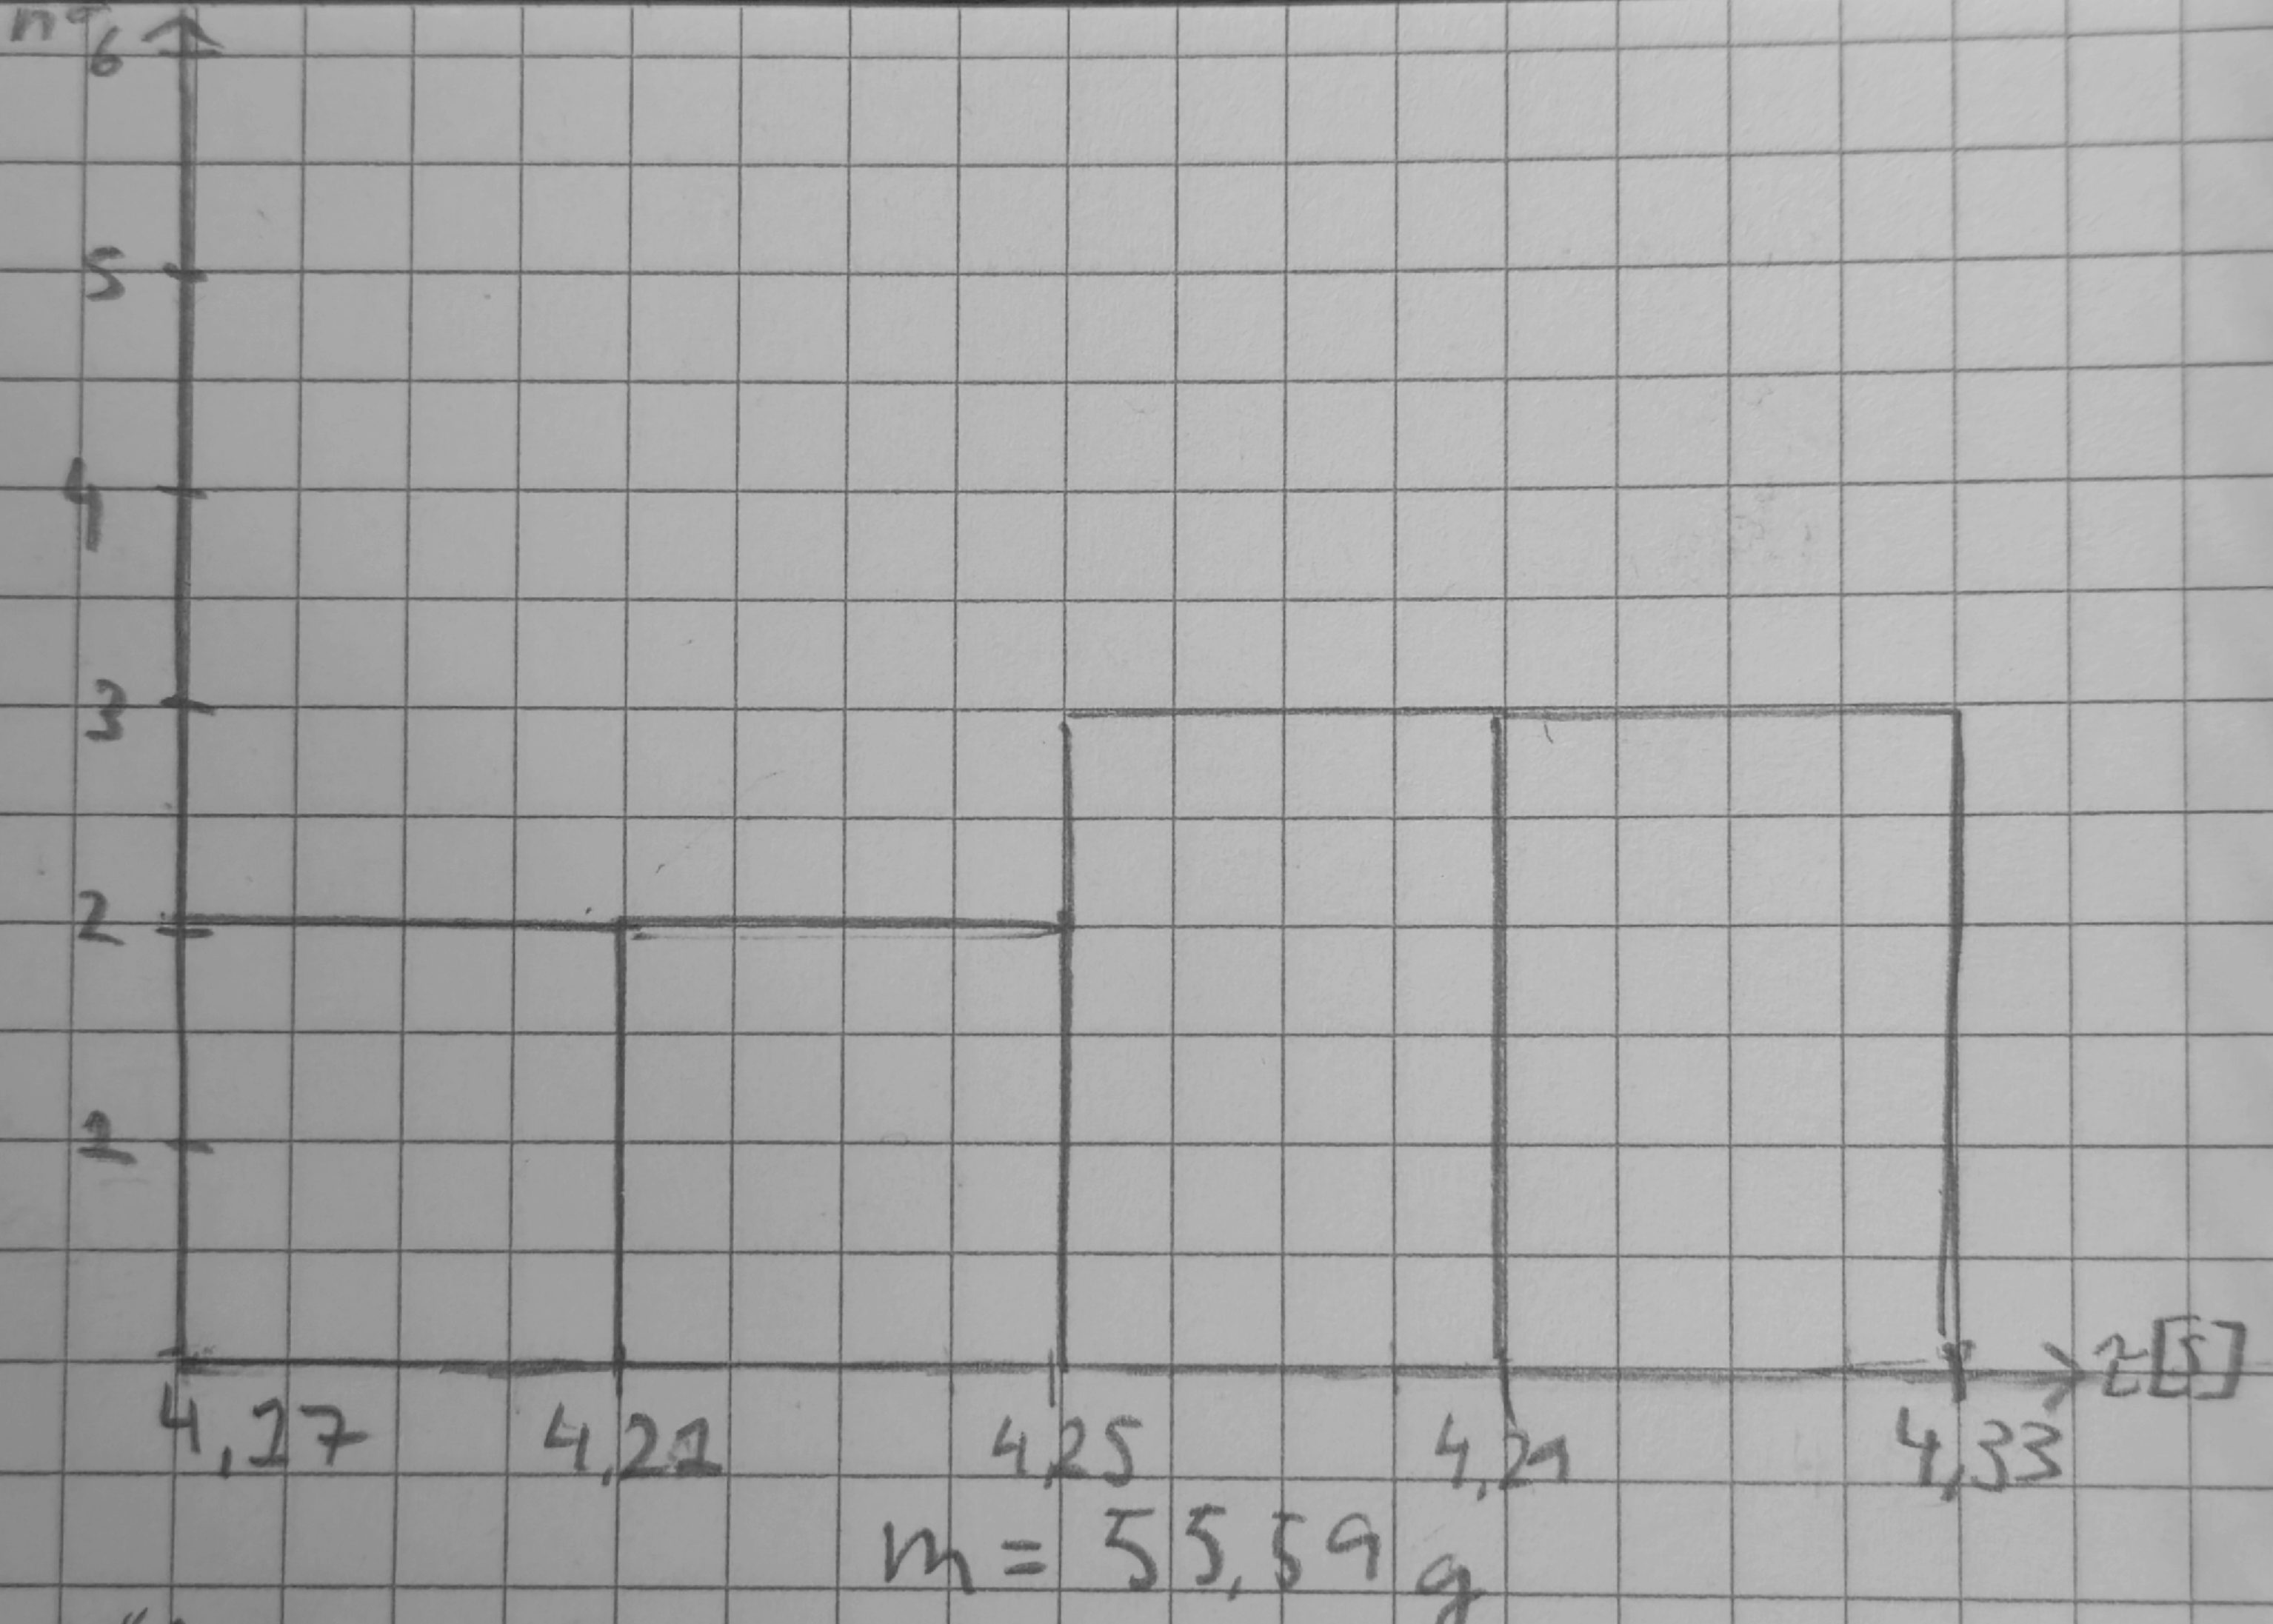
\includegraphics[width=\textwidth]{fotomolla/Molla 1/55.jpg}
        \caption{Misure con $m=\SI{55.59}{g}$}
    \end{minipage}
\end{figure}
\FloatBarrier

\subsection{Molla 2 Grafici}
\subsubsection{Metodo Statico}
\FloatBarrier
\begin{figure}[!ht]
    \centering
    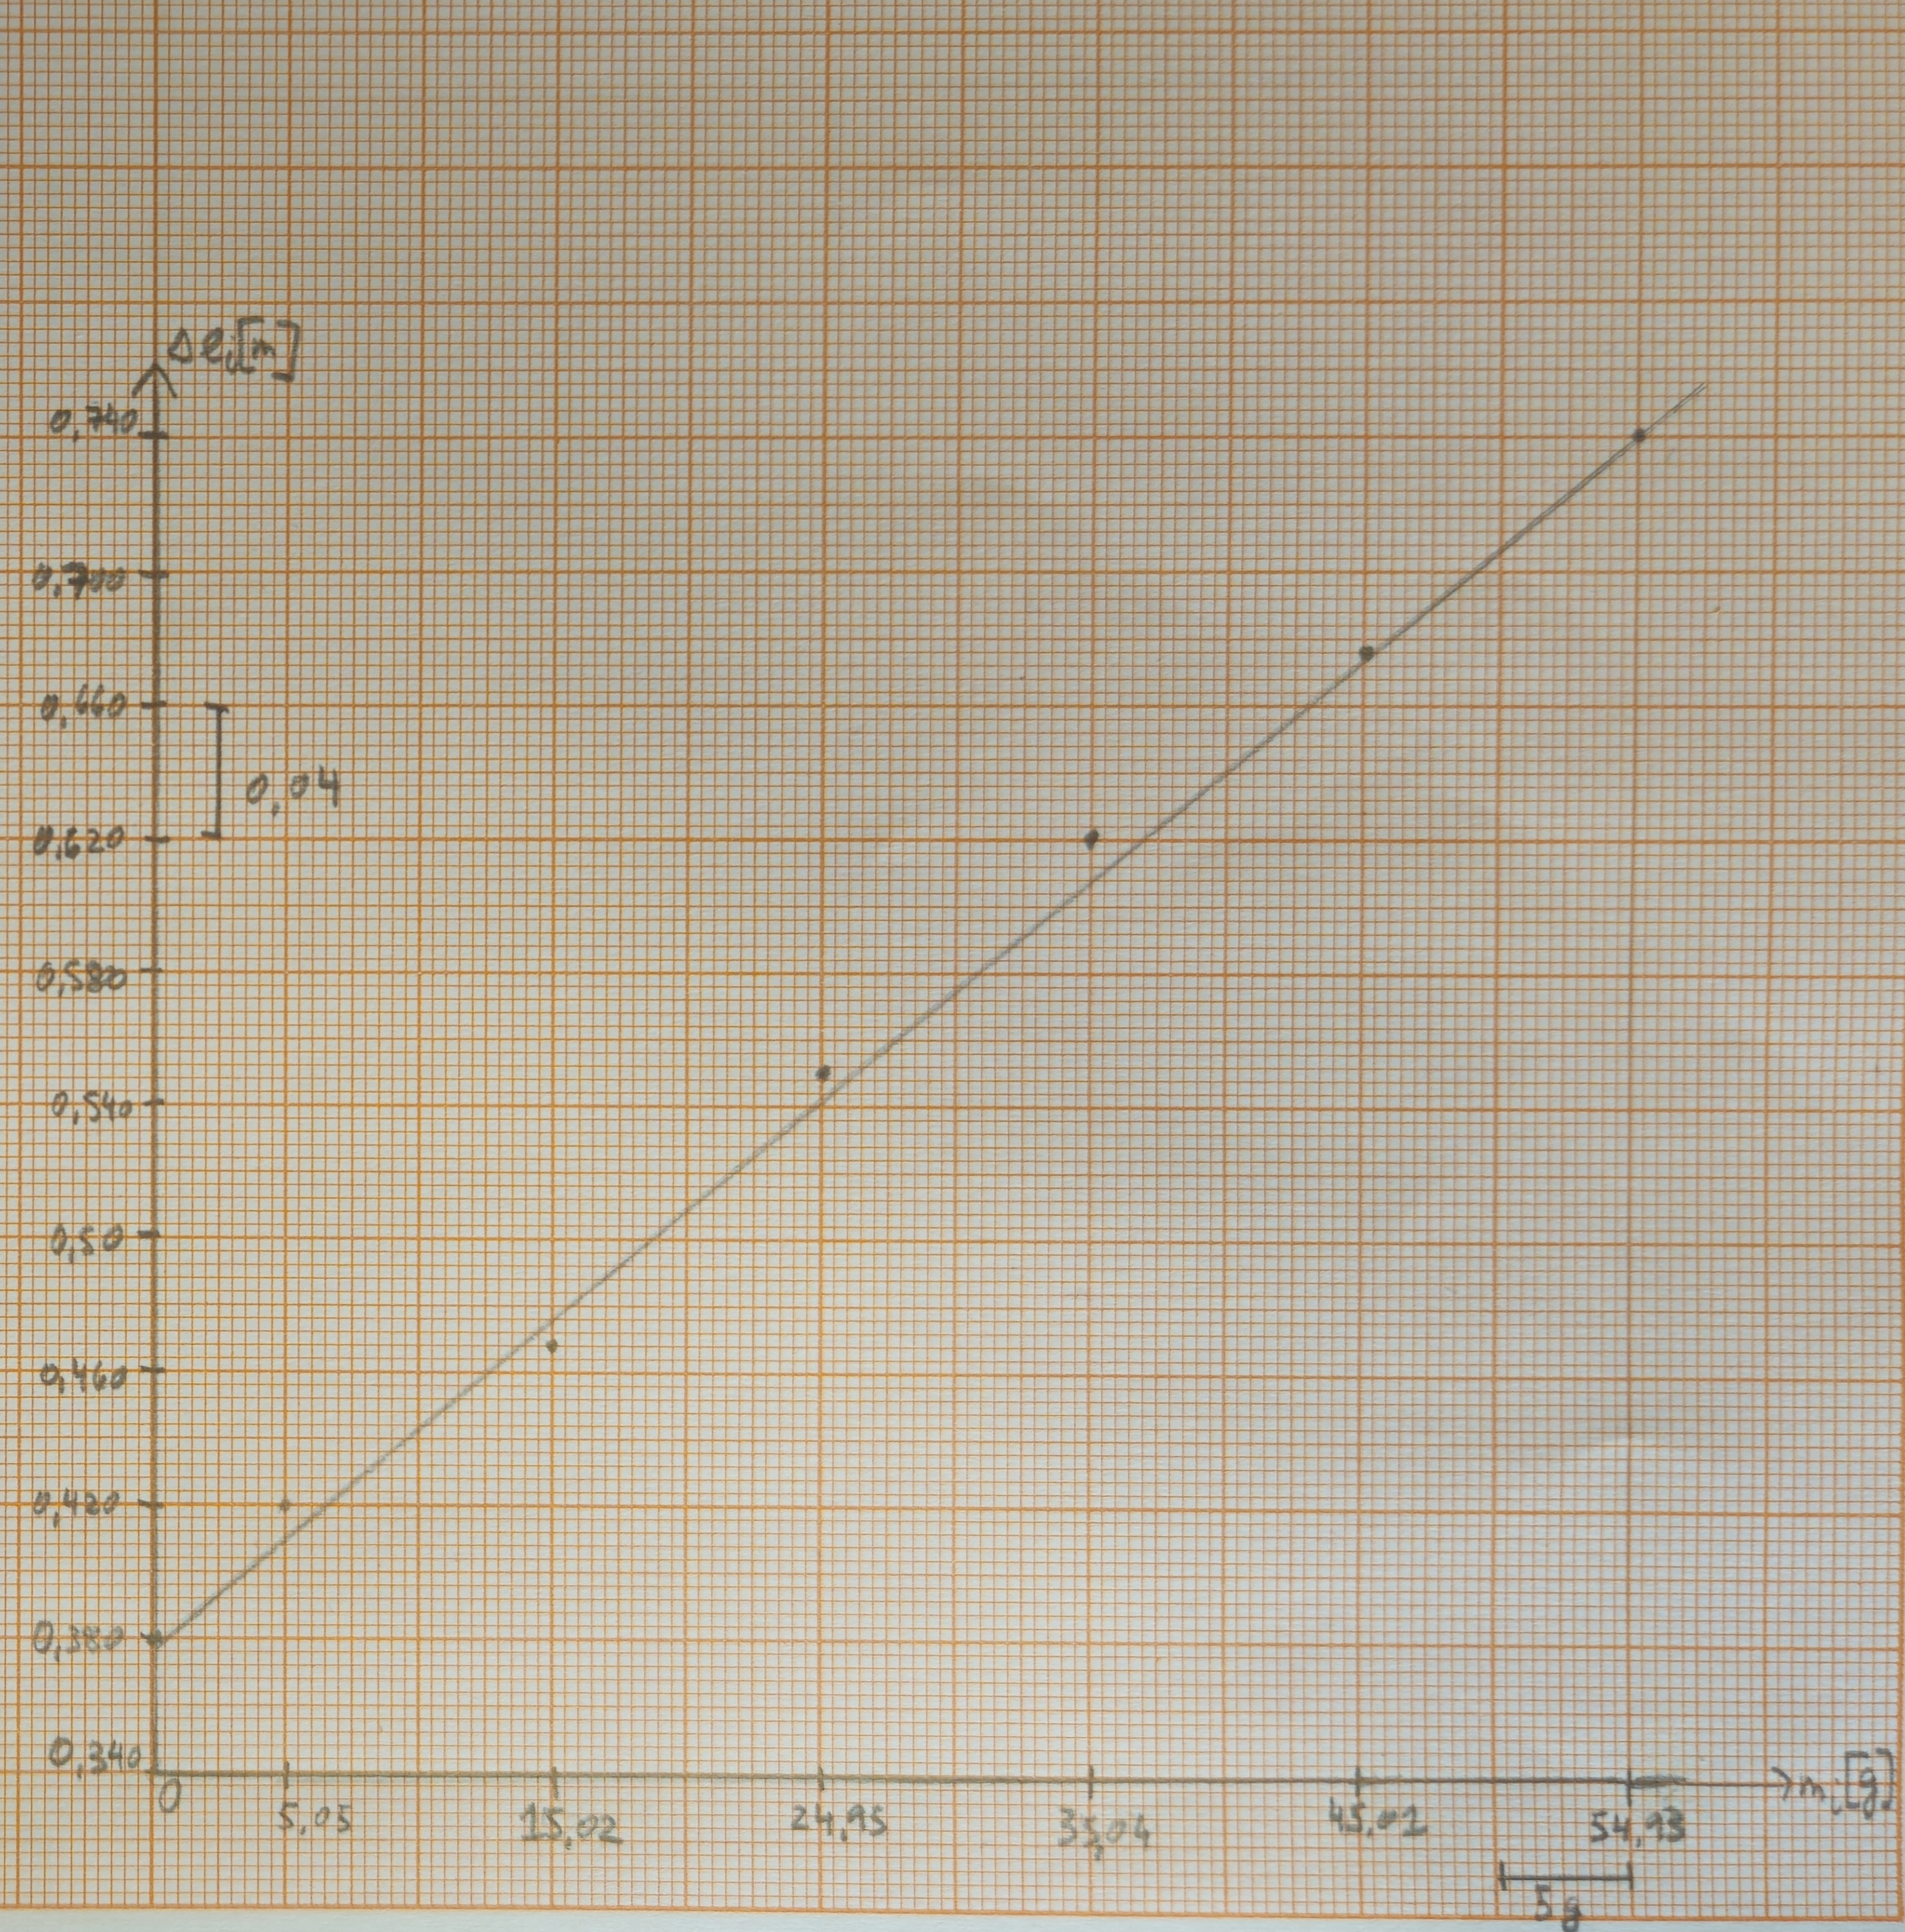
\includegraphics[width=0.6\textwidth]{fotomolla/Molla 2/m2statico_lm.jpg}
    \caption{Grafico di $\Delta L_i$ vs $M_i$}
\end{figure}

\begin{figure}[!ht]
    \centering
    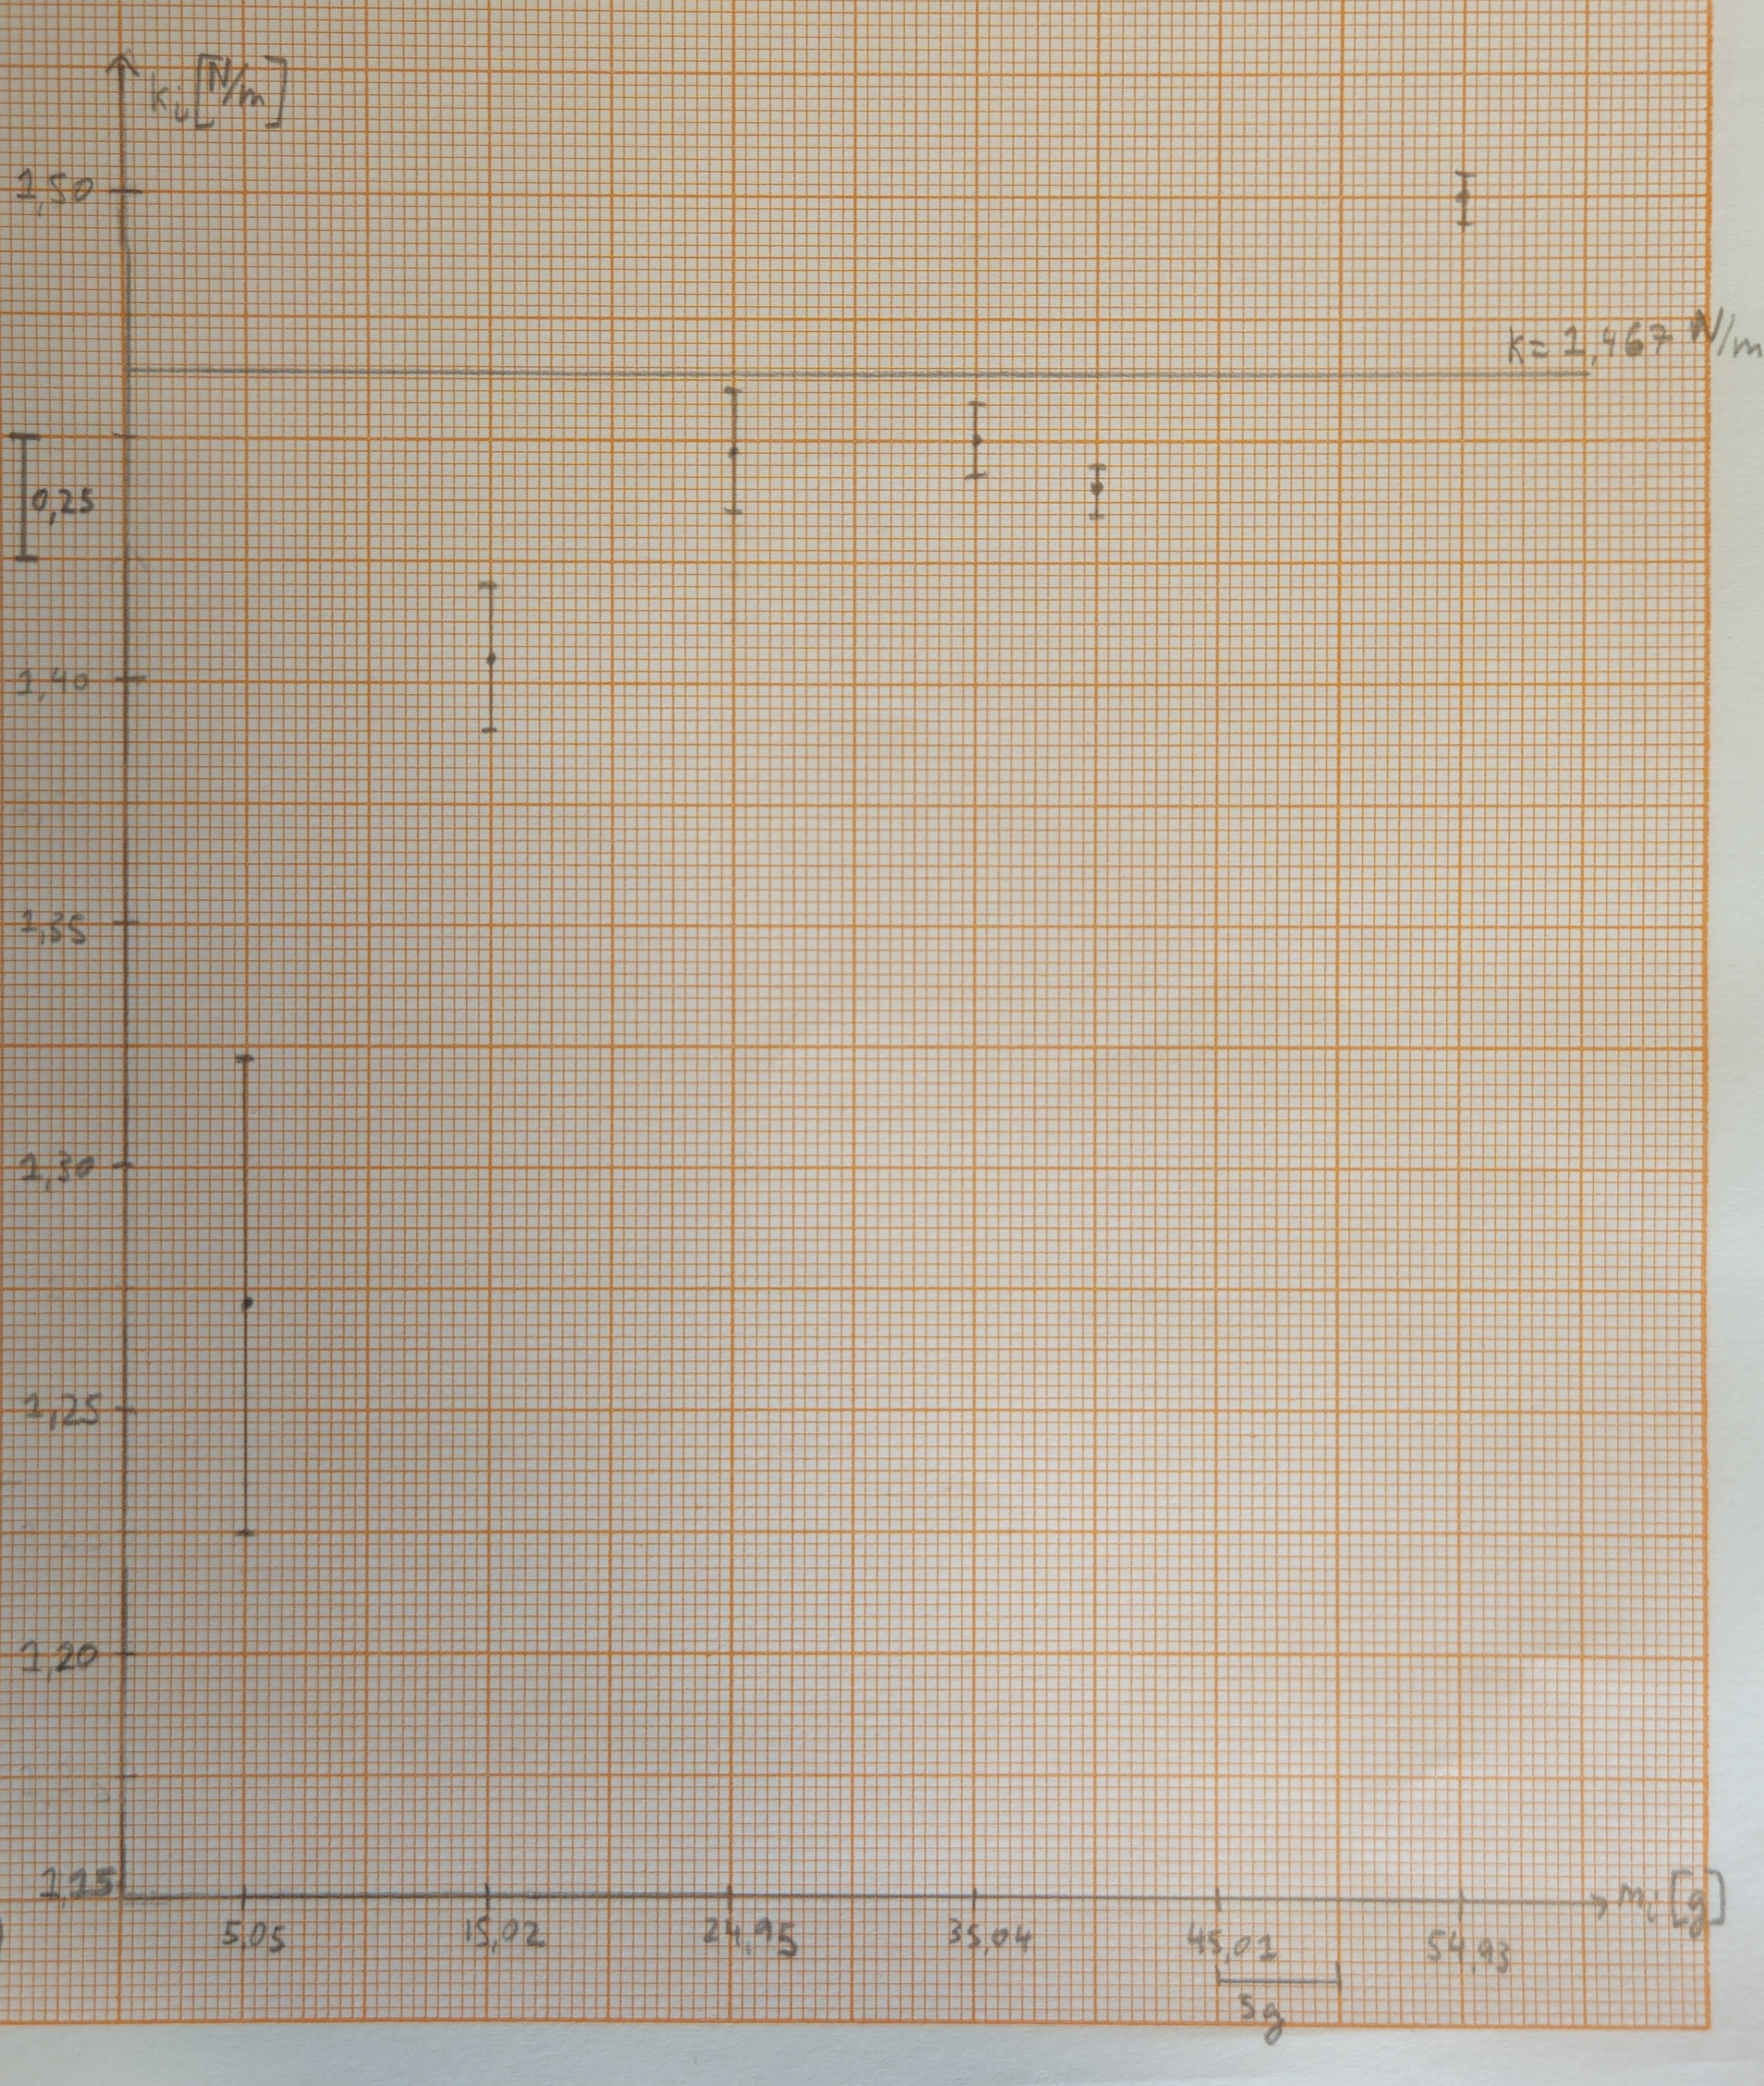
\includegraphics[width=0.6\textwidth]{fotomolla/Molla 2/m2statico_km.jpg}
    \caption{Grafico di $K_i$ vs $M_i$}
\end{figure}
\FloatBarrier

\subsubsection{Metodo Dinamico}
\begin{figure}[!ht]
    \centering
    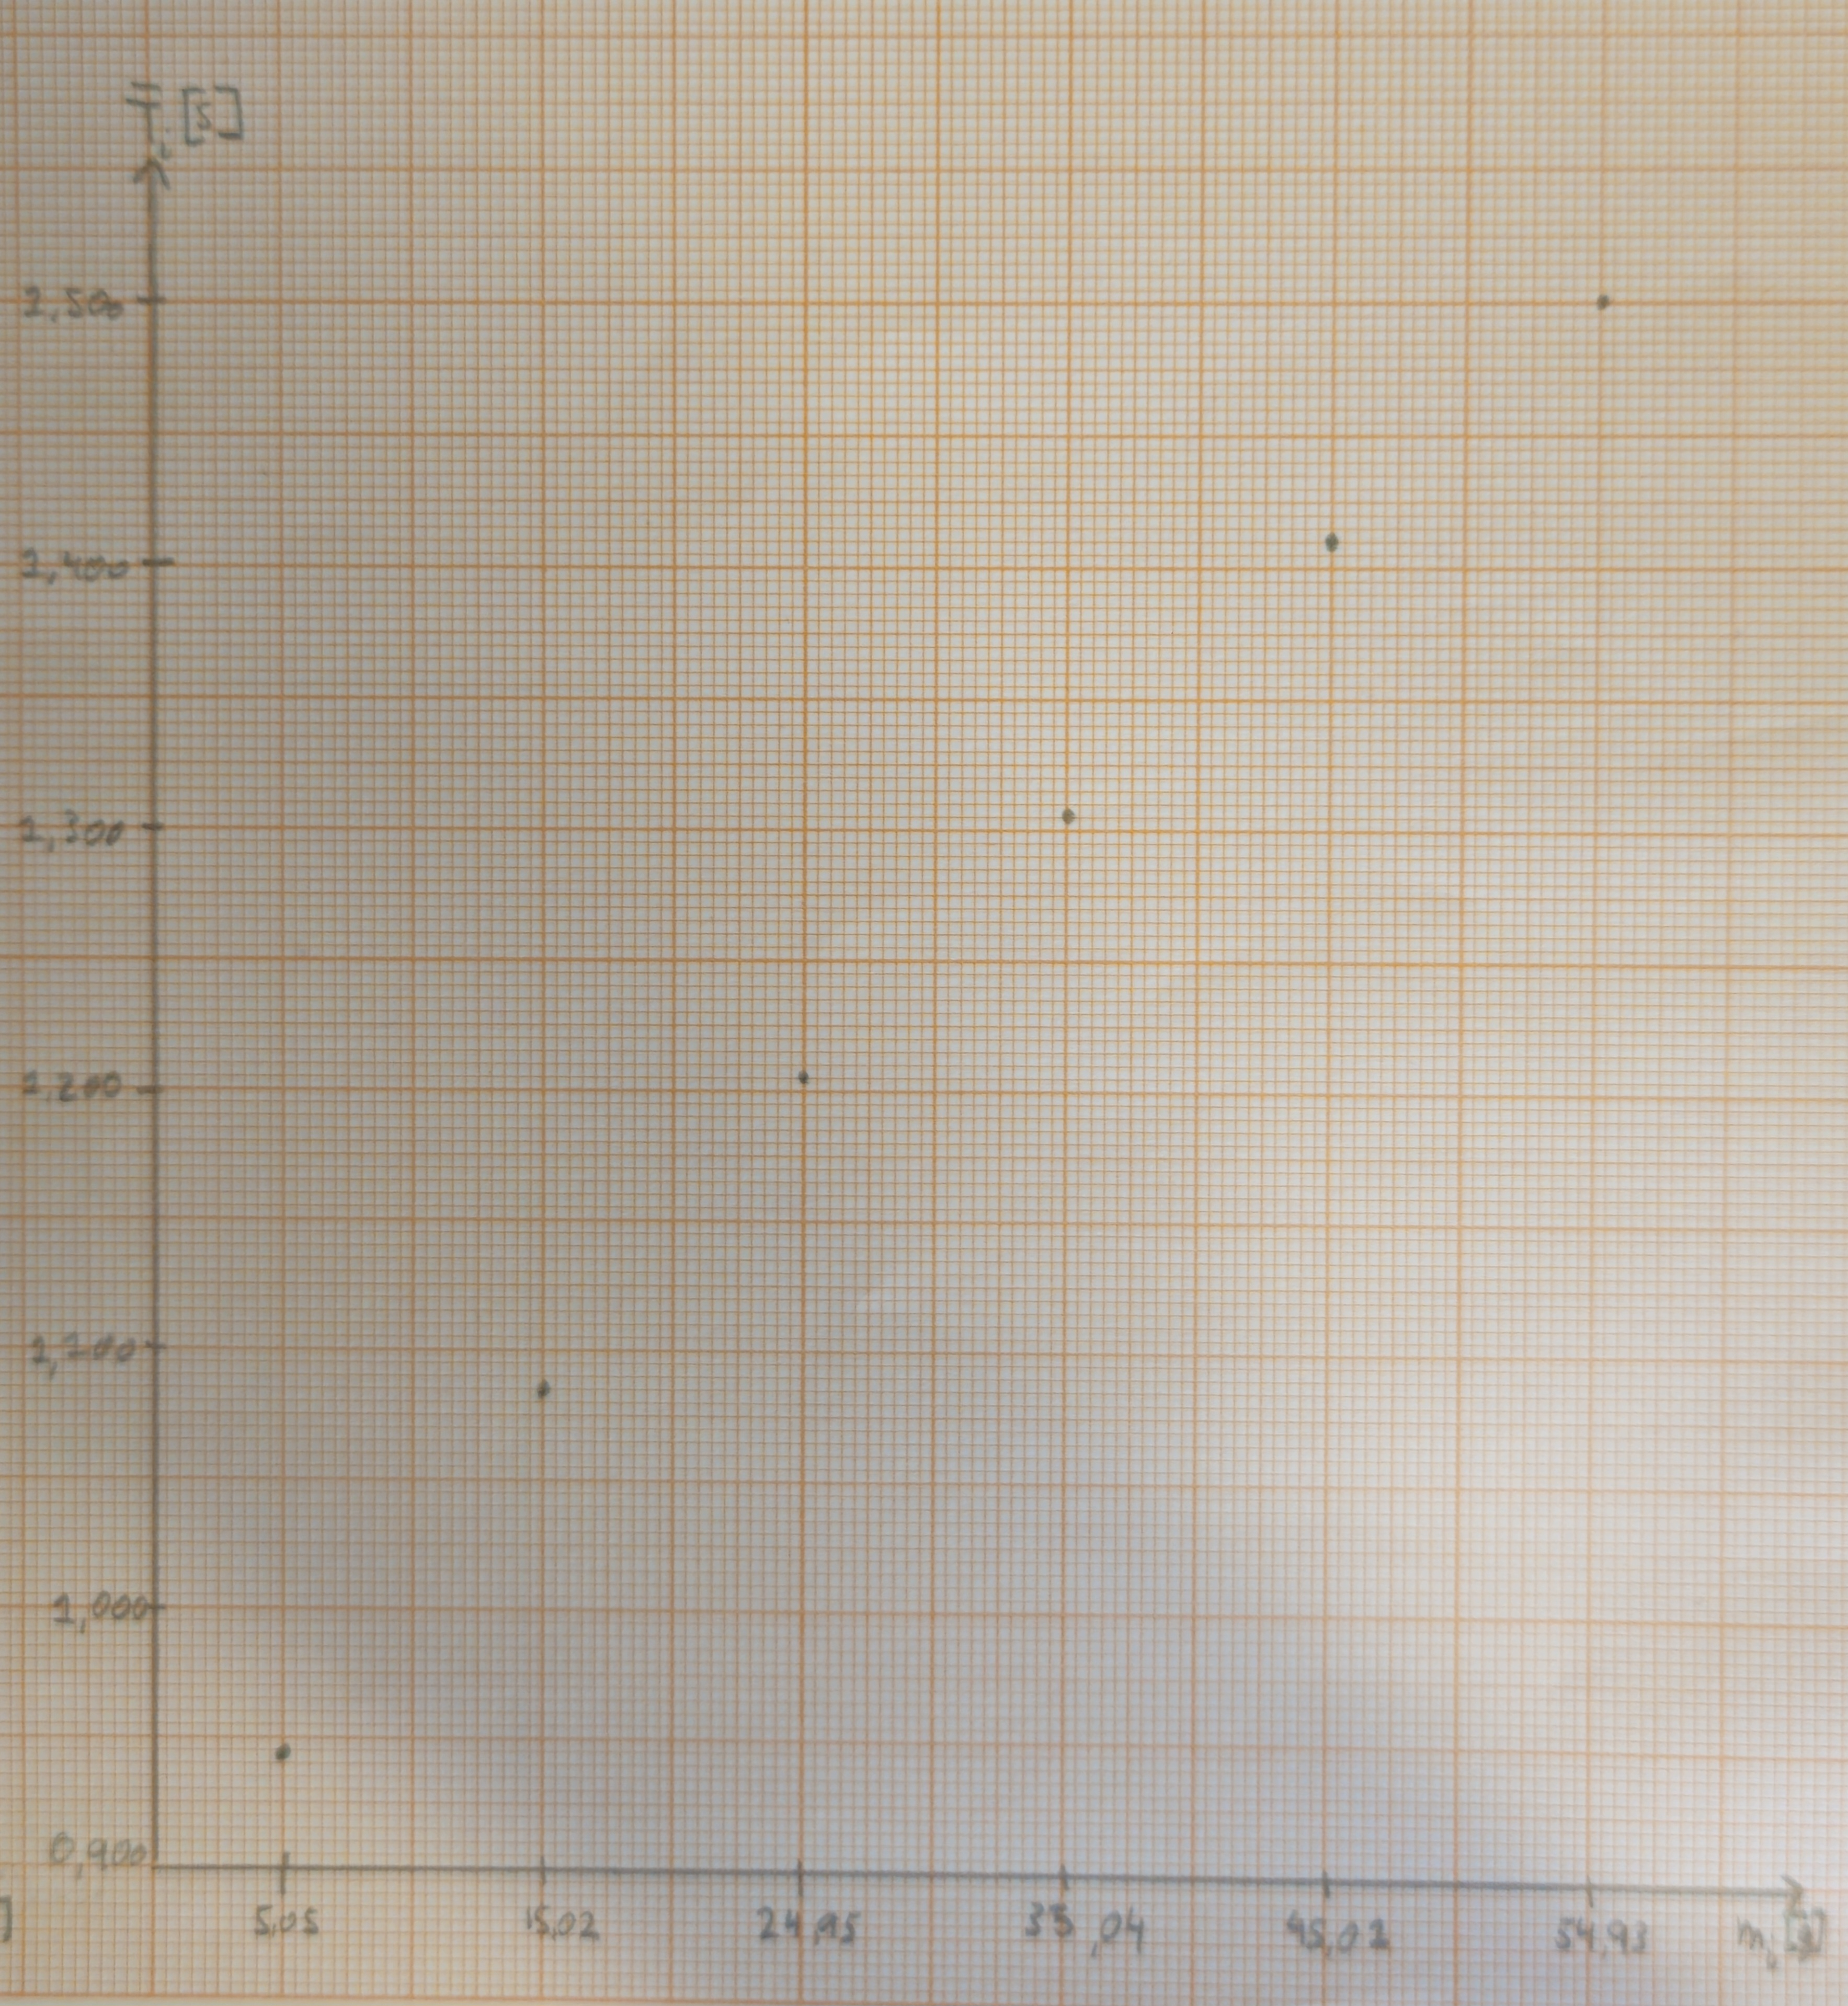
\includegraphics[width=0.6\textwidth]{fotomolla/Molla 2/m2dinamico_tm.jpg}
    \caption{Grafico di $\bar{T}_i$ vs $M_i$}
\end{figure}

\begin{figure}[!ht]
    \centering
    \includegraphics[width=0.6\textwidth]{fotomolla/Molla 2/m2dinamico_diffperiodo.jpg}
    \caption{Grafico di $k_2$ con modello differenza periodi}
\end{figure}

\begin{figure}[!ht]
    \centering
    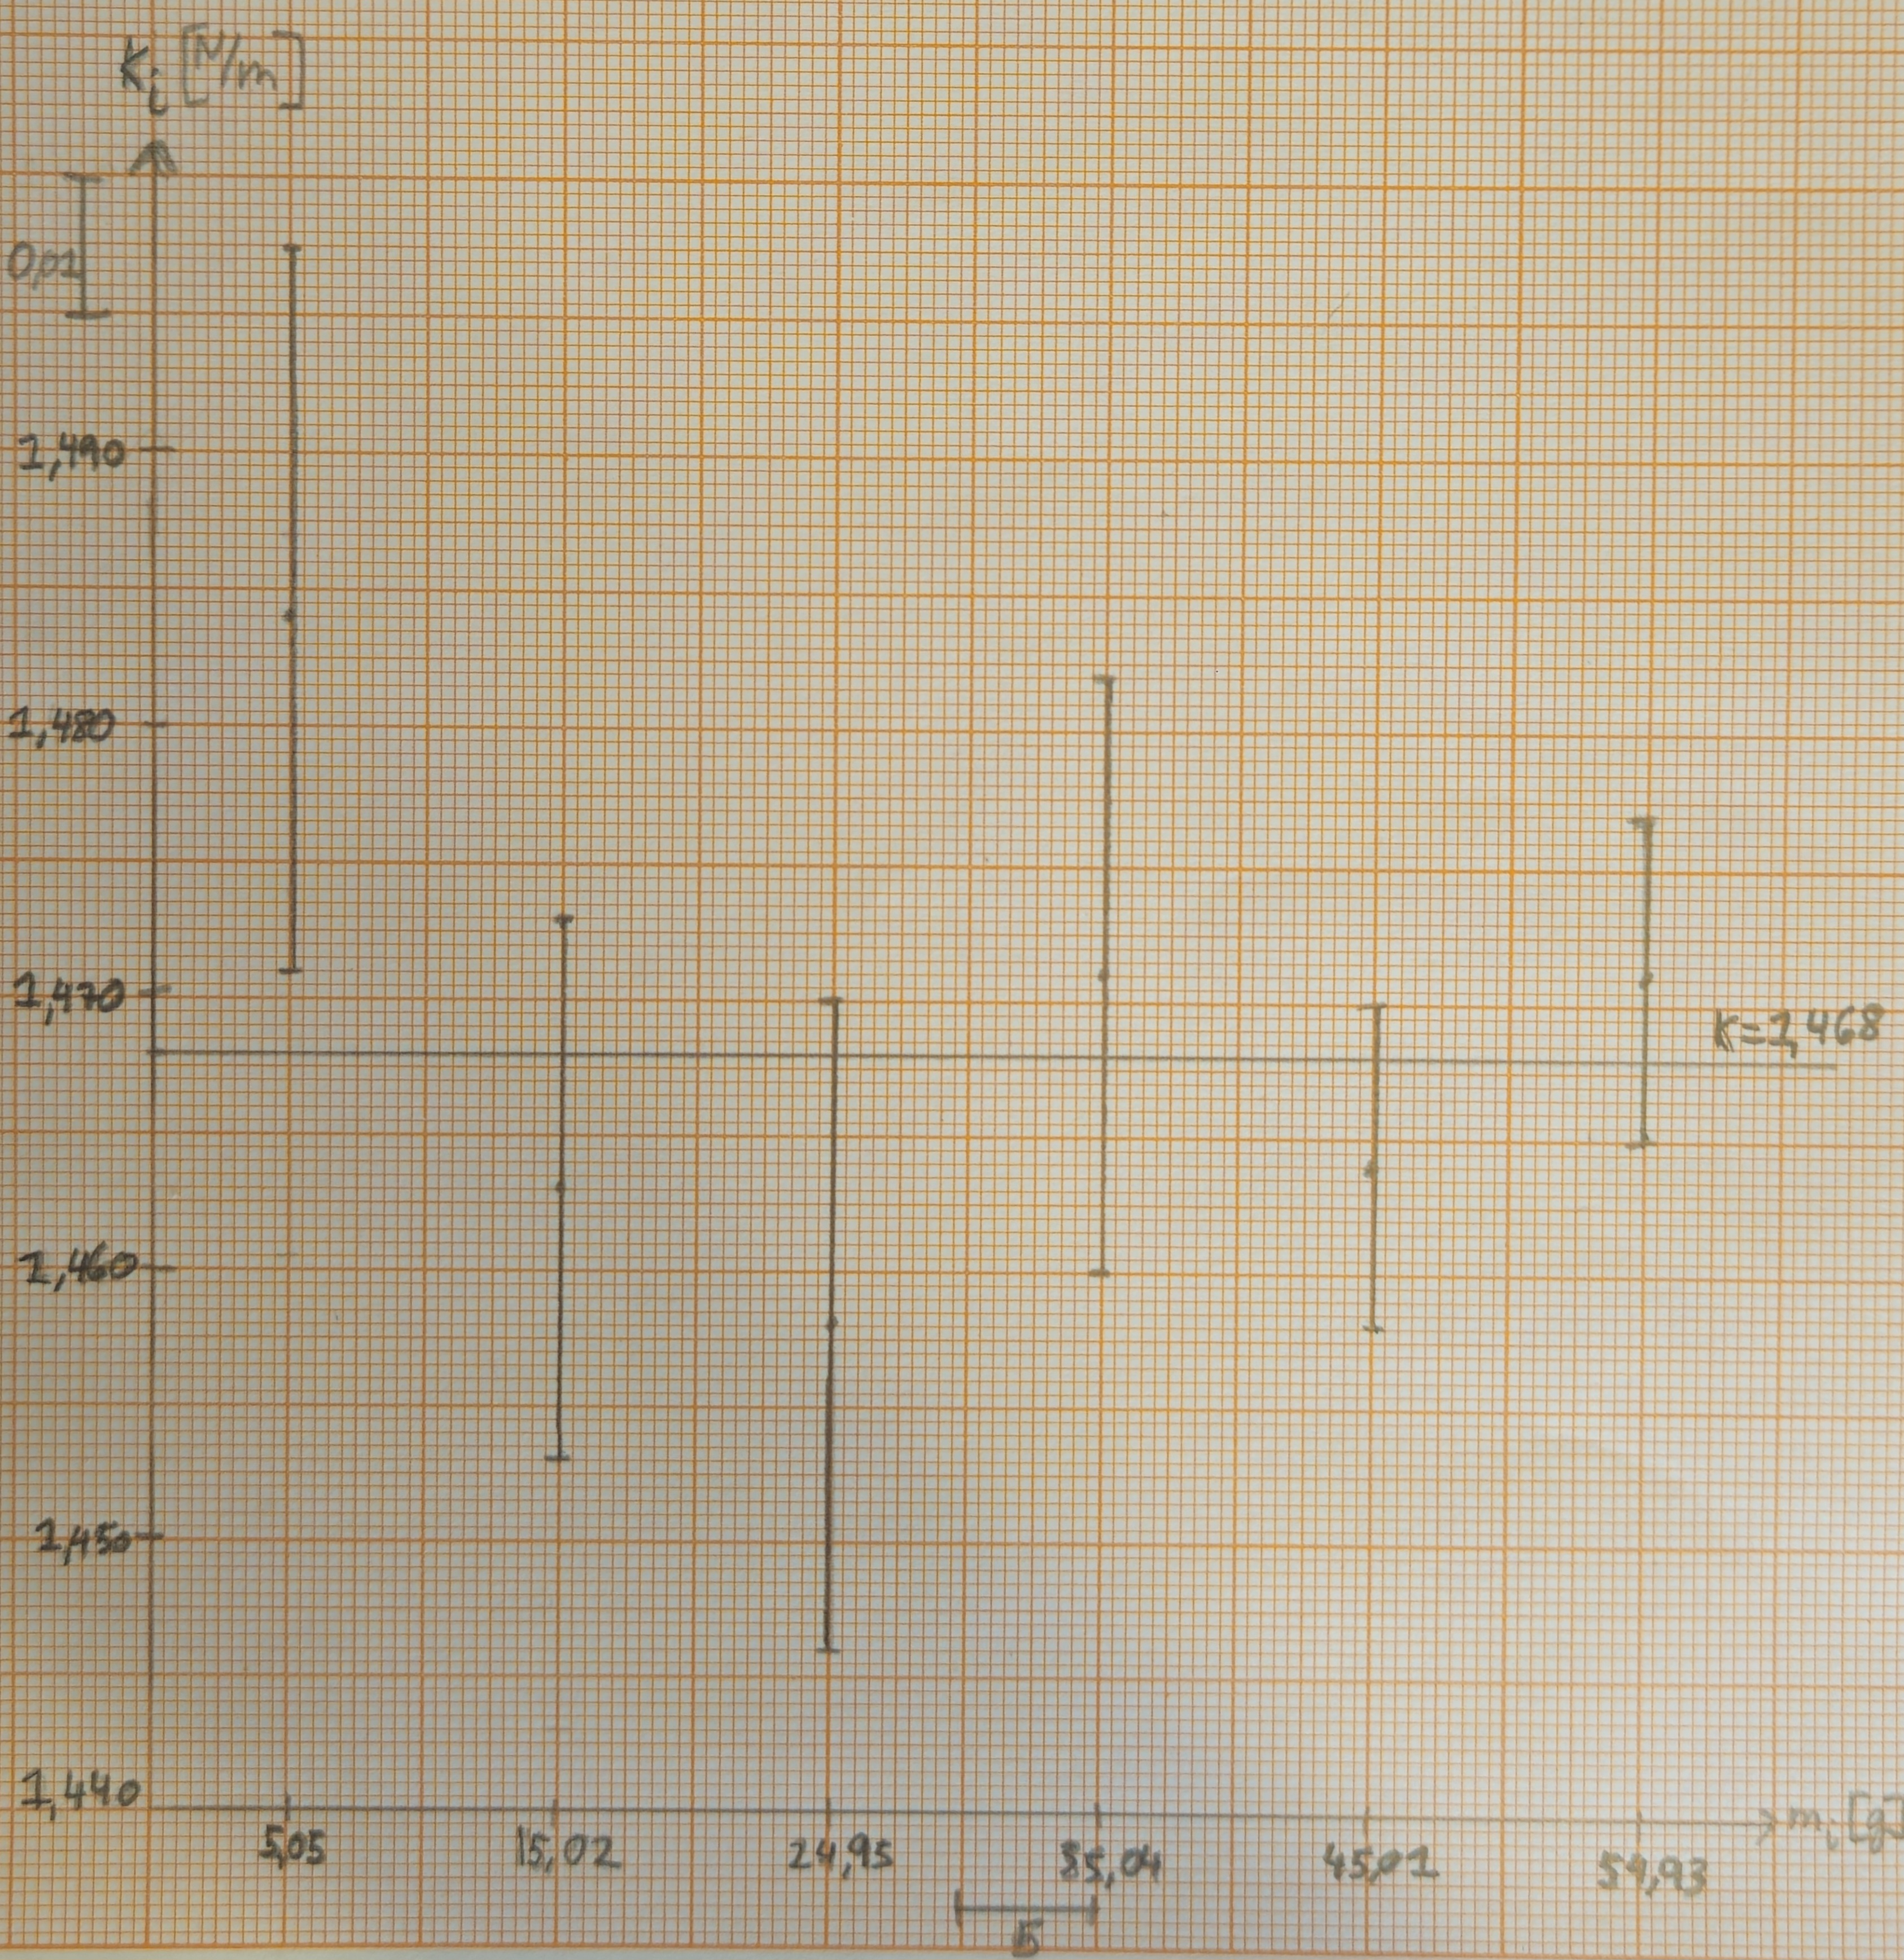
\includegraphics[width=0.6\textwidth]{fotomolla/Molla 2/m2dinamico_mefficace.jpg}
    \caption{Grafico di $k_2$ con modello $m_{eff}$}
\end{figure}
\FloatBarrier

\subsubsection{Istogrammi}
\begin{figure}[!ht]
    \centering
    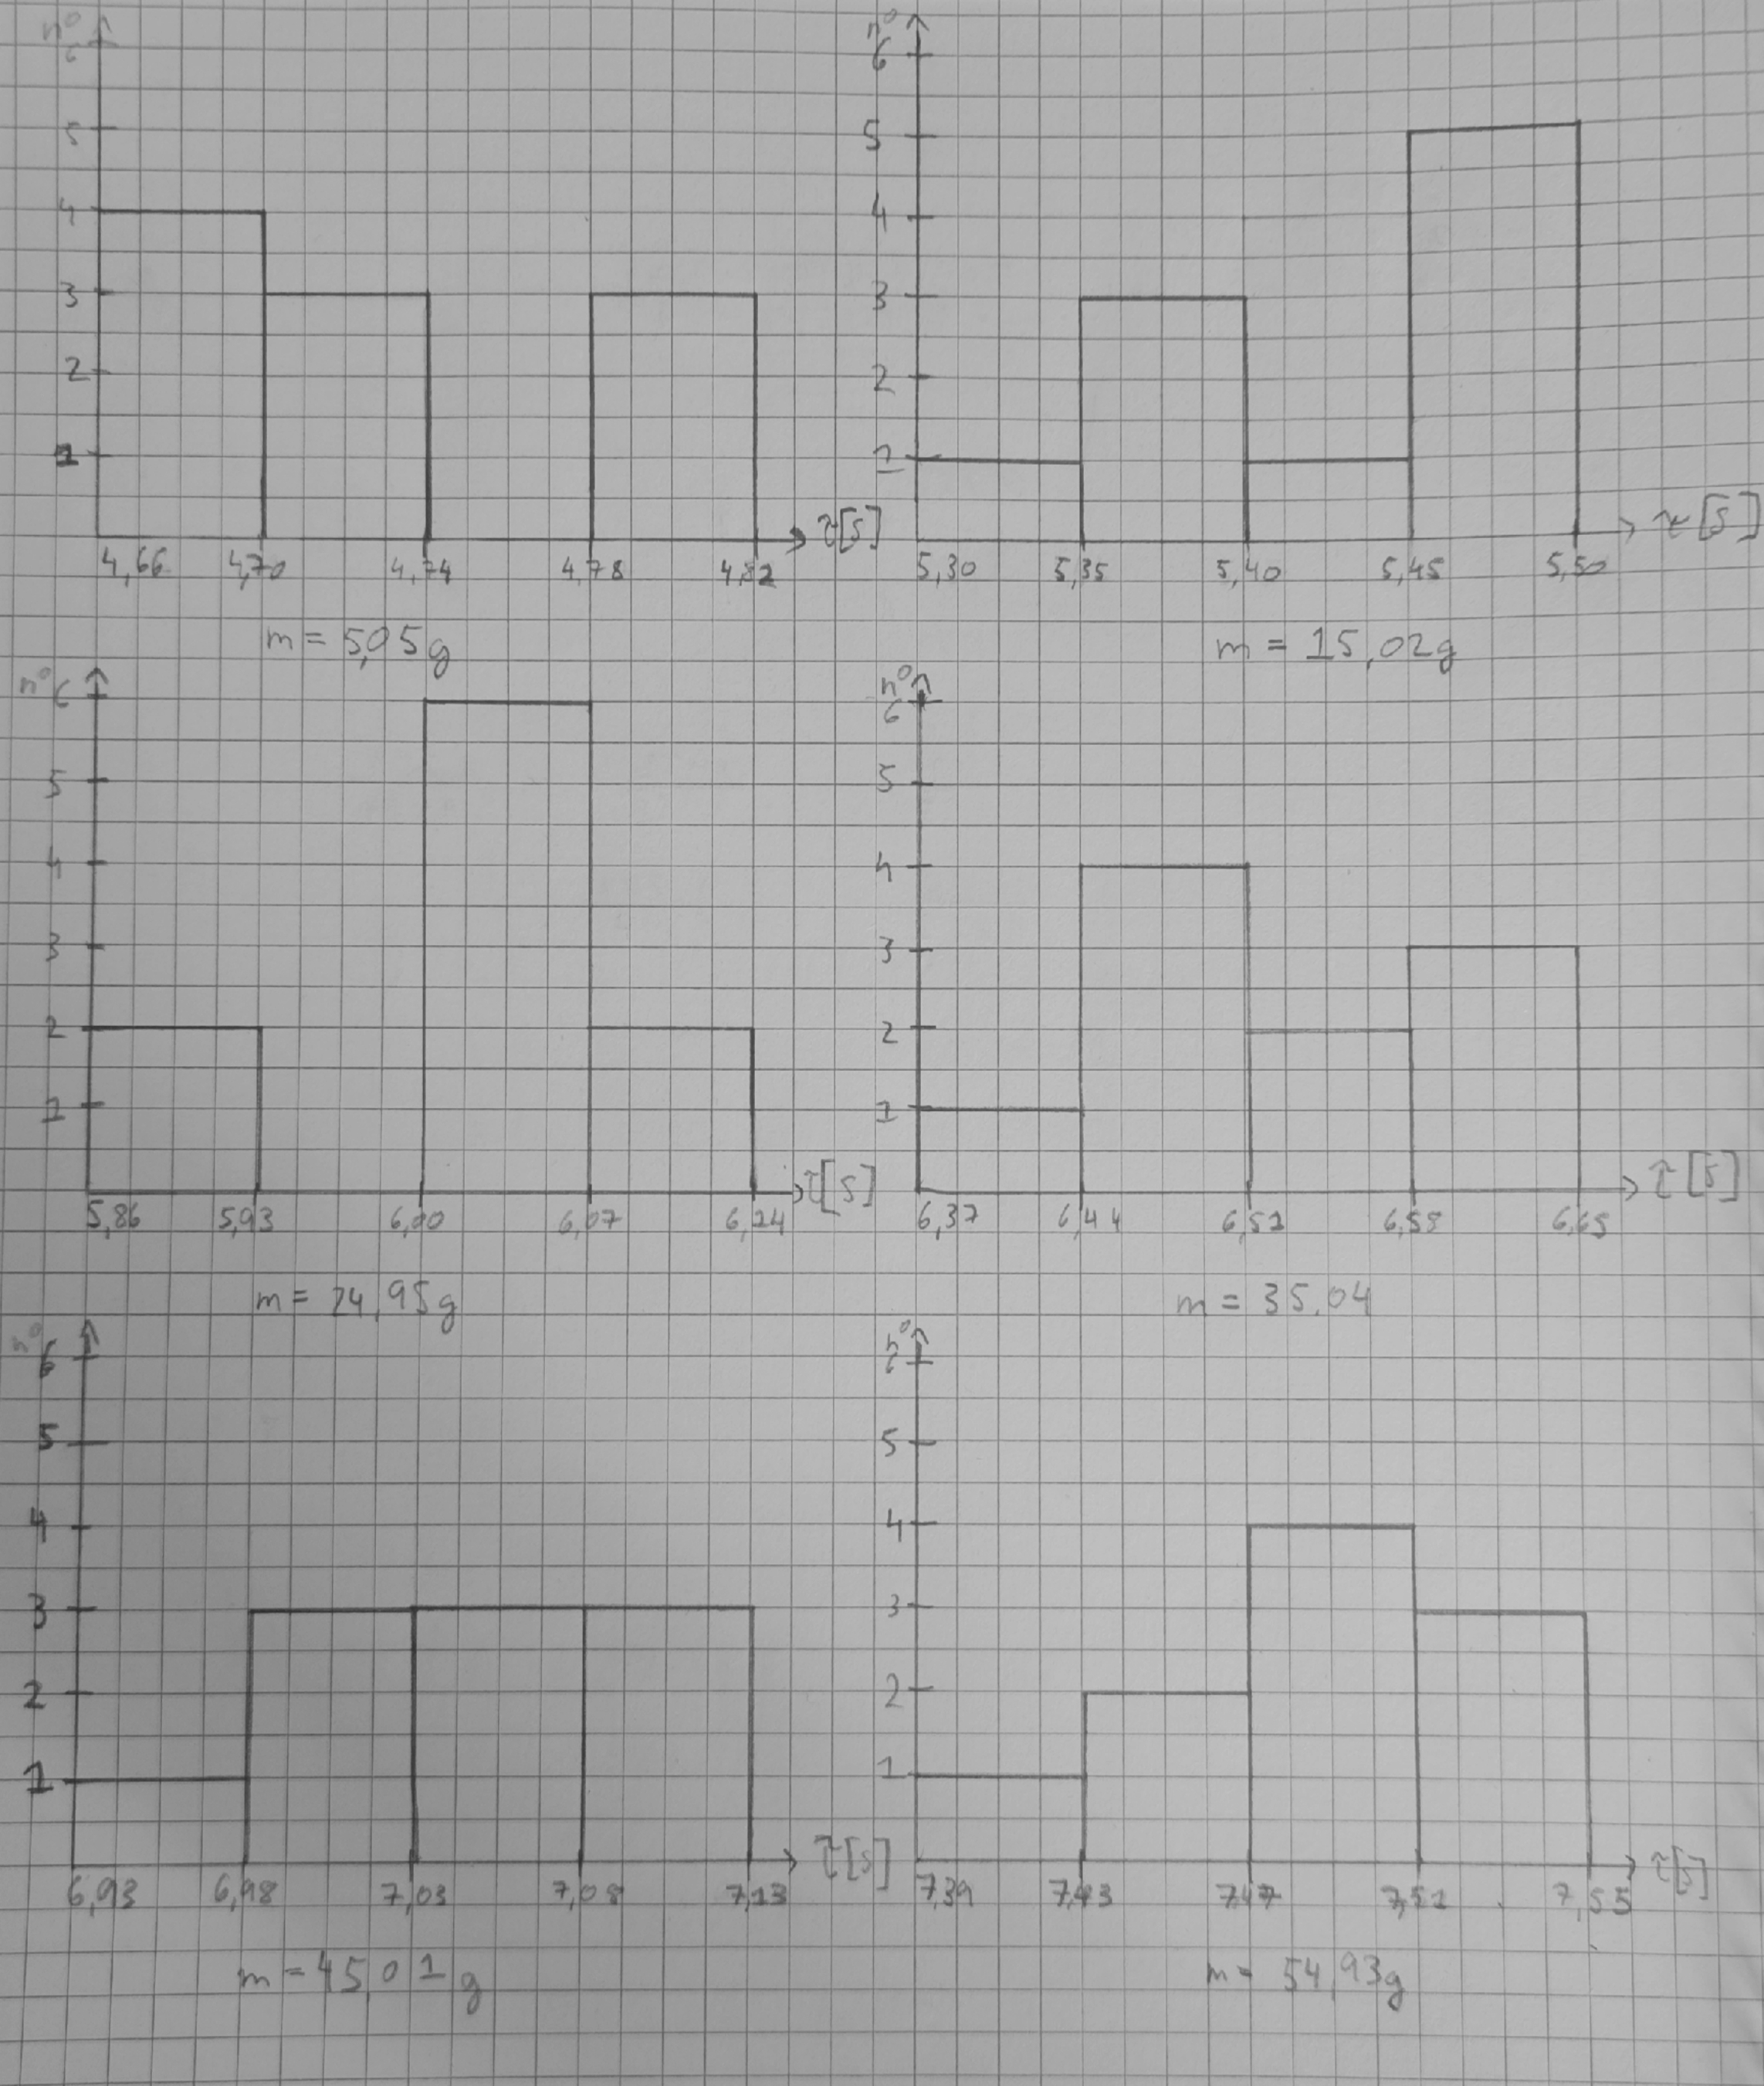
\includegraphics[width=\textwidth]{fotomolla/Molla 2/Molla 2.jpg}
    \caption{Istogrammi dei vari pesi}
\end{figure}

\end{document}